\renewcommand{\prevlecture}{10 }
\renewcommand{\thislecture}{11 }
\renewcommand{\nextlecture}{12 }

%
% Cover page
%

\title[PHYS 201 / Lecture \thislecture]
{
  PHYS 201 / Lecture \thislecture\\
  {\it Mutual and self inductance; \\ Inductance in circuits; RL, LC and RLC circuits}\\
}

\author[C.Andreopoulos] {
  Professor Costas Andreopoulos\inst{1,2}, {\it FHEA}
}
\institute[Liverpool/STFC-RAL] {
   \inst{1} University of Liverpool, Department of Physics\\
   \vspace{0.1cm}
   \inst{2} U.K. Research \& Innovation (UKRI), Science \& Technology Facilities Council,\\
            Rutherford Appleton Laboratory, Particle Physics Department\\
   \vspace{0.5cm}
   {\it {\color{magenta} Lectures delivered at the University of Liverpool, 2020-21}}\\
   \vspace{0.2cm}
}
\date{\today}

\titlegraphic{
  
\includegraphics[height=25px]{./images/logo/liverpool.png}
  \hspace{3px}
  
\includegraphics[height=30px]{./images/logo/ral.png}
}


\begin{frame}[plain]
  \titlepage
\end{frame}

% ------------------------------------------------------------------------------
% ------------------------------------------------------------------------------

%
% Revision of previous lecture
%

\renewcommand{\lecturesummarytitle}{Revision }

\renewcommand{\summarizedlecture}{10 }

%
%
%

\begin{frame}{Lecture \summarizedlecture - \lecturesummarytitle}

{\small

We studied the most general case of Maxwell's equations:\\

\setlength{\extrarowheight}{12pt}
\setlength{\arraycolsep}{5pt}

 \begin{center}
 {

  \begin{table}[H]
    \begin{tabular}{|l|c|c|}
      \hline
        \multicolumn{3}{|l|} {
          {\color{magenta}
           {\bf Dynamic case in matter}
          }
        }\\
      \hline
      {\bf Gauss's law} &
        $\displaystyle \oint \vec{D} d\vec{S} = \int \rho_f d\tau = Q_f$   &
        $\displaystyle \vec{\nabla} \cdot \vec{D} = \rho_f$ \\

      {\bf Faraday's law} &
        $\displaystyle \oint \vec{E} d\vec{\ell} = -\frac{\partial}{\partial t} \int \vec{B} d\vec{S} \Rightarrow$ &
        $\displaystyle \vec{\nabla} \times \vec{E} = -  \frac{\partial \vec{B}}{\partial t}$ \\
      &
        $\displaystyle \oint \vec{E} d\vec{\ell} = -\frac{d\Phi_B}{dt}$ & \\

      no magn. monopoles &
        $\displaystyle  \oint \vec{B} d\vec{S} = 0$ &
        $\displaystyle  \vec{\nabla} \cdot \vec{B} = 0$ \\

      {\bf Ampere's law} &
        $\displaystyle \oint \vec{H} d\vec{\ell} = \int_{S} \Big( \vec{j} + \frac{\partial \vec{D}}{\partial t}\Big) d\vec{S} \Rightarrow$ &
        $\displaystyle \vec{\nabla} \times \vec{H} = \vec{j}_f + \frac{\partial \vec{D}}{\partial t}$ \\
      &
        $\displaystyle \oint \vec{H} d\vec{\ell} = I_f + \frac{d\Phi_D}{dt}$ & \\
      \hline
    \end{tabular}
  \end{table}

 }
 \end{center}
}

\end{frame}

%
%
%

\begin{frame}{Lecture \summarizedlecture - \lecturesummarytitle (cont'd)}

\begin{itemize}

\item As we did in vacuum, we studied Maxwell's equations in matter (for time-dependent fields)
          and in the absence of sources and we saw that they give rise to EM waves:
          \begin{equation*}
             \vec{\nabla}^{2} \vec{E} = \mu \epsilon \frac{\partial^{2} \vec{E}}{\partial t^{2}} \;\;\;\; and \;\;\;\;
             \vec{\nabla}^{2} \vec{B} = \mu \epsilon \frac{\partial^{2} \vec{B}}{\partial t^{2}}
         \end{equation*}

\item Speed of EM waves in matter: $\displaystyle u = \frac{1}{\sqrt{\epsilon \mu}}$
         \begin{itemize}
         {\small
               \item EM waves in matter propagate slower than EM waves in vacuum
               \item $\displaystyle u = \frac{c}{n}$ where
                         $\displaystyle n = \frac{\sqrt{\epsilon \mu}}{\sqrt{\epsilon_0 \mu_0}}$
                         is the index of refraction of the material.
         }
         \end{itemize}

\item We introduced a complex representation of EM waves starting from de Moivre's theorem
          and embedding the known EM wave properties (EM waves are always {\bf transverse} and
          {\bf mutually perpendicular}):
          \begin{equation*}
                \vec{E}(\vec{r},t) = E_0  e^{i (\vec{k} \vec{r} -\omega t)} \hat{n}
                 \;\;\; and \;\;\;
                \vec{B}(\vec{r},t) =
                  \frac{E_0}{c}  e^{i ( \vec{k} \vec{r} -\omega t)} \Big( \hat{k} \times \hat{n} \Big) =
                  \frac{1}{c}  \Big( \hat{k} \times \vec{E} \Big)
          \end{equation*}

\end{itemize}

\end{frame}

%
%
%

\begin{frame}{Lecture \summarizedlecture - \lecturesummarytitle (cont'd)}

\begin{itemize}

\item We also studied EM wave polarization and practical applications.

\item Finally, we studied the electrodynamic boundary conditions:\\
          \vspace{0.2cm}
         For the electric field:
         \begin{equation*}
               \epsilon_1 E_1^{\perp} = \epsilon_2 E_2^{\perp}  \;\;\;\; and \;\;\;\;
                E_1^{\parallel} = E_2^{\parallel}
         \end{equation*}
         For the magnetic field:
         \begin{equation*}
               B_1^{\perp} = B_2^{\perp} \;\;\;\; and \;\;\;\;
               \frac{1}{\mu_1} B_1^{\parallel} = \frac{1}{\mu_2} B_2^{\parallel}
         \end{equation*}

\item We used the above conditions to study what happens when
          an EM wave crosses the {\bf boundary between two transparent media}\\
          \vspace{0.2cm}
          Two cases:
          \begin{itemize}
               \item Normal incidence
               \item Oblique incidence (general case / home study)
          \end{itemize}
\end{itemize}

\end{frame}


%
%
%

\begin{frame}{Lecture \summarizedlecture - \lecturesummarytitle (cont'd)}

\begin{itemize}
{\small
\item Maxwell's equations in most general form (time-dependent fields in matter)
    \begin{itemize}
     {\scriptsize
          \item You should know both the integral and differential forms.
          \item You should know all variations of these equations and be able to derive
                    one from another (dynamic $\rightarrow$ static, matter $\rightarrow$ vacuum)
          \item No marks given for writing the wrong set of equations, even if they are all
                    similar and interconnected.\\
    }
    \end{itemize}

\item You should be able to show that Maxwell's equations (in vacuum or in matter) in
          absence of sources describe EM waves

\item You should know how the wave equation and the EM waves are different in vacuum and in transparent media.

\item You should know how to use the complex representation of waves.

\item You should know (and be able to derive) the electrodynamic boundary conditions,
          and you should be able to use them to study reflection and transmission at normal and oblique incidence.

\item You should remember the fundamental laws of geometrical optics and what is Brewster's angle.
}
\end{itemize}

\end{frame}


%
% Plan for this lecture
%

\begin{frame}{Plan for Lecture \thislecture}

\begin{itemize}
\item Mutual and self inductance
\item Inductance in circuits
  \begin{itemize}
      \item RL circuits
      \item LC circuits
      \item RLC circuits
  \end{itemize}
\end{itemize}

\end{frame}

% ------------------------------------------------------------------------------
% ------------------------------------------------------------------------------

%
%
%

\begin{frame}{Mutual inductance}

Consider two closed conductor loops (1 and 2) at rest, as shown.

\begin{columns}
  \begin{column}{0.55\textwidth}
    \begin{center}
       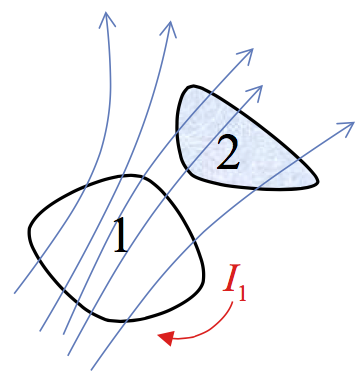
\includegraphics[width=0.90\textwidth]{./images/schematics/mutual_inductance_1.png}\\
     \end{center}
  \end{column}
  \begin{column}{0.45\textwidth}
     \begin{itemize}
        \item A steady current $I_1$ circulates in loop 1.
        \vspace{0.4cm}
        \item The current $I_1$ generates a magnetic field $B_1$.
        \vspace{0.4cm}
        \item Some of the flux of the magnetic field $B_1$ goes through the surface $S_2$
     \end{itemize}
  \end{column}
\end{columns}

\end{frame}

%
%
%

\begin{frame}{Mutual inductance}


The magnetic field due to the current $I_1$ flowing in loop 1 is given by the Biot-Savart law:
\begin{equation*}
  \vec{B}_1 = \frac{\mu_0}{4\pi} I_1 \oint_{L_1} \frac{d\vec{\ell_1} \times \vec{r}}{r^3}
\end{equation*}

The flux through the surface of loop 2, of the magnetic field $\vec{B}_1$ produced by loop 1 is:
\begin{equation*}
  \Phi_2 = \int_{S_2} \vec{B}_1 \cdot d\vec{S_2}
\end{equation*}

Therefore:
\begin{equation*}
  \Phi_2 = \int_{S_2}
      {\color{magenta} \Big\{ }
        \frac{\mu_0}{4\pi} I_1 \oint_{L_1} \frac{d\vec{\ell_1} \times \vec{r}}{r^3}
      {\color{magenta} \Big\} } \cdot d\vec{S_2}
\end{equation*}

\end{frame}

%
%
%

\begin{frame}{Mutual inductance}

\begin{equation*}
  \Phi_2 = \int_{S_2}
      {\color{magenta} \Big\{ }
        \frac{\mu_0}{4\pi} I_1 \oint_{L_1} \frac{d\vec{\ell_1} \times \vec{r}}{r^3}
      {\color{magenta} \Big\} } \cdot d\vec{S_2} \Rightarrow
\end{equation*}

\begin{equation*}
  \Phi_2 = {\color{magenta}\bigg\{ }
                   \frac{\mu_0}{4\pi} \int_{S_2} \Big\{ \oint_{L_1} \frac{d\vec{\ell_1} \times \vec{r}}{r^3} \Big\} \cdot d\vec{S_2}
                 {\color{magenta}\bigg\} }  I_1 \Rightarrow
\end{equation*}

\begin{equation*}
   {\color{magenta} \Phi_2 = M_{21}  I_1 }
\end{equation*}

where
\begin{equation*}
  M_{21}  =  \frac{\mu_0}{4\pi} \int_{S_2} \Big\{ \oint_{L_1} \frac{d\vec{\ell_1} \times \vec{r}}{r^3} \Big\} \cdot d\vec{S_2}
\end{equation*}

\vspace{0.3cm}

{\bf The flux $\Phi_2$ is proportional to $I_1$}.\\
\vspace{0.2cm}

The constant of proportionality ($M_{21}$) is known as {\bf mutual inductance}.\\
$M_{21}$  is a {\bf purely geometrical} factor.

\end{frame}

%
%
%

\begin{frame}{Mutual inductance}

A simpler formula for $M_{21}$ can be derived by expressing the magnetic field
$\vec{B}$ in terms of its vector potential $\vec{A}$ and using Stokes's theorem.

\vspace{0.2cm}

\begin{columns}
  \begin{column}{0.40\textwidth}
    \begin{center}
       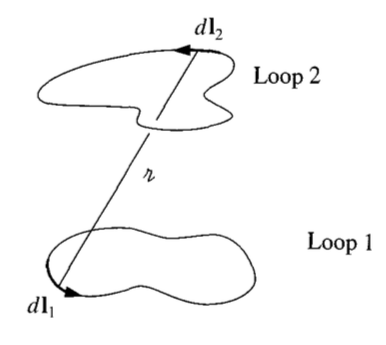
\includegraphics[width=0.80\textwidth]{./images/schematics/mutual_inductance_2.png}\\
     \end{center}
  \end{column}
  \begin{column}{0.60\textwidth}
    \begin{equation*}
      M_{21}  =  \frac{\mu_0}{4\pi} \oint_{L_1} \oint_{L_2} \frac{d\vec{\ell_1} \cdot d\vec{\ell_2}}{r}
    \end{equation*}
     This is the {\bf Neumann formula} (without proof):
     It involves a double line integral - one integration is around loop 1 and the other integration is around loop 2.
  \end{column}
\end{columns}

It reveals 2 important things about the mutual inductance:
\begin{itemize}
{\small
   \item It is purely geometrical, as we have already discussed.
            (It has to do only with the shape, size and relative positions of the 2 loops.)
   \item It is {\bf unchanged if one switches the roles of loop 1 and 2}
       \begin{itemize}
       {\small
             \item So $M_{21}$ = $M_{12}$ !
       }
       \end{itemize}
}
\end{itemize}

\end{frame}

%
%
%

\begin{frame}{Mutual inductance}

Mutual inductance unchanged if one switches the roles of loop 1 and 2.\\

\vspace{0.2cm}

\begin{columns}
  \begin{column}{0.30\textwidth}
    \begin{center}
       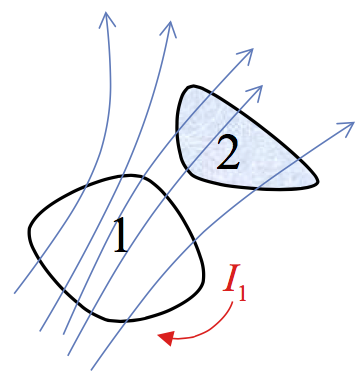
\includegraphics[width=0.99\textwidth]{./images/schematics/mutual_inductance_1.png}\\
     \end{center}
  \end{column}
  \begin{column}{0.70\textwidth}
  {\small
         This is a {\bf remarkable conclusion}!\\
         \vspace{0.2cm}
         \underline{Whatever} the shapes and positions of the loops,
         the flux through loop 2 when we run a current I around loop 1 is
         identical to the flux through loop 1 when we run the same current around loop 2.
         \begin{equation*}
               \Phi_2 = M_{21}  I_1 \xRightarrow{I_1 = I}  \Phi_2 = M_{21}  I
         \end{equation*}
         \begin{equation*}
               \Phi_1 = M_{12}  I_2 \xRightarrow{I_2 = I; M_{12} = M_{21}}  \Phi_1 = M_{12}  I \Rightarrow
               {\color{magenta}
                     \Phi_1 = \Phi_2
               }
         \end{equation*}
  }
  \end{column}
\end{columns}

\begin{columns}
  \begin{column}{0.20\textwidth}
    \begin{center}
       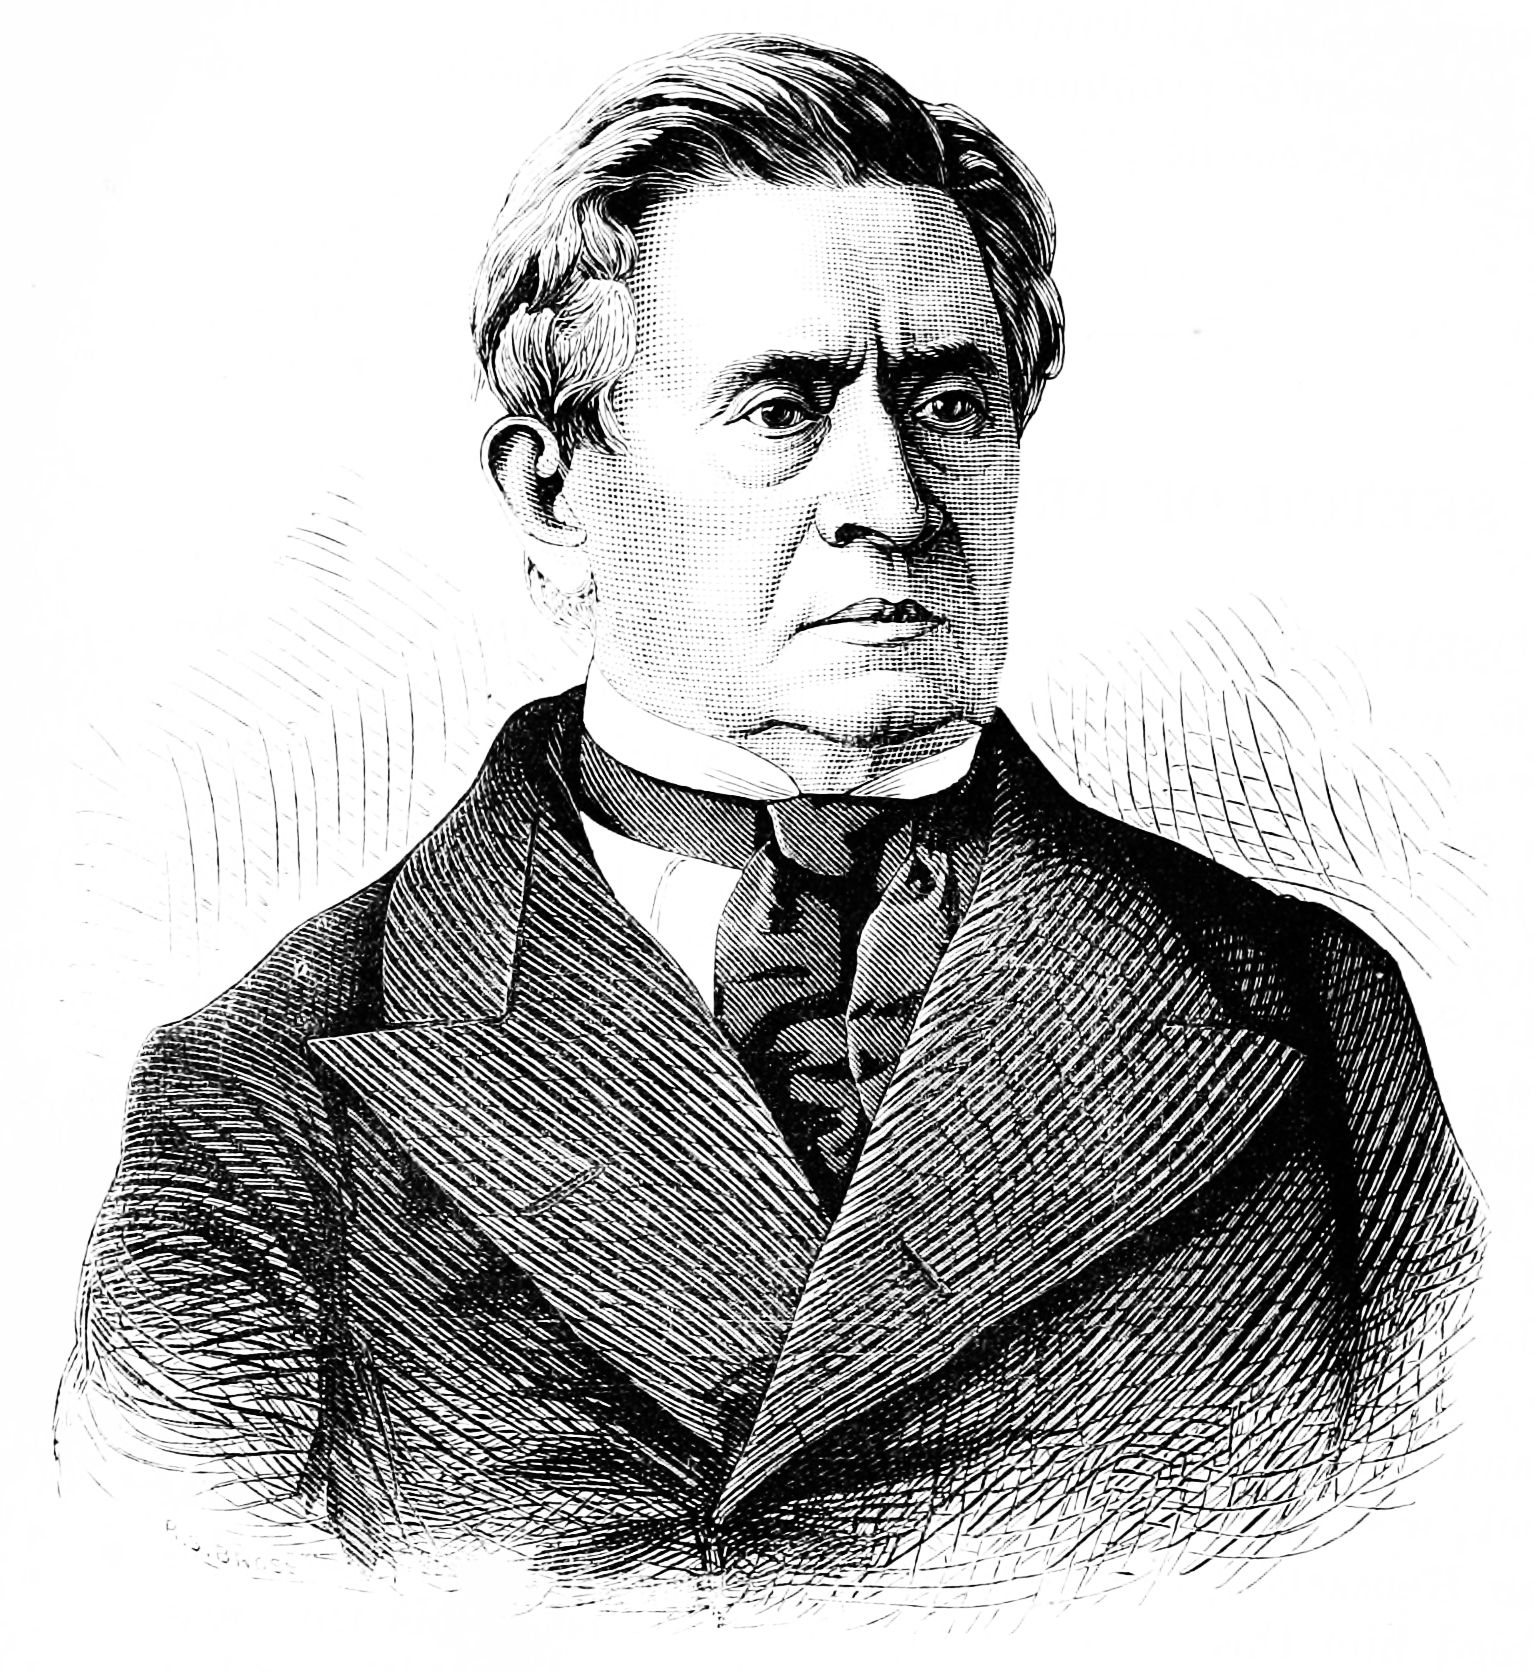
\includegraphics[width=0.70\textwidth]{./images/people/henry.jpg}\\
       {\tiny J.Henry, 1797-1878}
     \end{center}
  \end{column}
  \begin{column}{0.80\textwidth}
  {\small
        From now on I will drop the indices: $M_{21}$ = $M_{12}$ = {\color{magenta} $M$ }\\
        The SI unit of the mutual inductance is the {Henry} (H)
        \begin{itemize}
              \item Named in honour of Joseph Henry.
              \item 1 H = $\displaystyle \frac{Wb}{A}$ = $\displaystyle \frac{V \cdot s}{A}$
        \end{itemize}
  }
  \end{column}
\end{columns}


\end{frame}

%
%
%

\begin{frame}{Mutual inductance}

Before, $I_1$ was a steady current, so the field $\vec{B}_1$ did not change with time.\\
The conducting loops were fixed in their positions so $\Phi_2$ was also constant.\\

\vspace{0.3cm}

Now, let’s consider {\bf what happens if $I_1$ varies}:
\begin{itemize}
   \item  time-varying current $\rightarrow$ time-varying magnetic field
   \item  time-varying magnetic field $\rightarrow$  time-varying flux through loop 2.
\end{itemize}

\vspace{0.3cm}

Faraday's law tells us that this time-varying flux through loop 2 will
generate an EMF in loop 2:

\begin{equation*}
  \mathcal{E}_2 = - \frac{d\Phi_2}{dt} = - \frac{d}{dt} \Big( M I_1 \Big) = - M \frac{dI_1}{dt}
\end{equation*}

\vspace{0.2cm}

Varying the current in a loop, {\bf causes an EMF} (and a current) {\bf in a nearby loop},
although the two loops are not connected electrically.
\begin{itemize}
   \item They are connected ``magnetically''
\end{itemize}

\end{frame}



%
%
%

\begin{frame}{Self inductance}

Varying the current in loop 1, varies the magnetic field and thus the magnetic
flux passing through loop 1 itself!\\

\vspace{0.3cm}
Again, we can write that:

\begin{equation*}
  \mathcal{E}_1 = - L \frac{dI_1}{dt}
\end{equation*}

where the constant of proportionality is called {\bf self-inductance of the loop}
(or simply inductance) and it is denoted with L (in honour of H.Lenz).

\end{frame}

%
%
%

\begin{frame}{Self inductance / ``Back EMF''}

As we have seen, if you try to change the current in a loop,
there will be an EMF developed in that same loop as a result of the current change.
\begin{equation*}
  \mathcal{E} = - L \frac{dI}{dt}
\end{equation*}

Remember Lenz's law: {\bf  Nature dislikes changes in the magnetic flux.}

\vspace{0.2cm}

The EMF developed in the loop, as a result of the current change,
will be such so as to {\bf oppose the current change}. \\
For that reason, it is called {\bf back EMF} (or {\bf counter EMF}).

\vspace{0.2cm}

{\bf Inductance  may be thought of as electromagnetic inertia}.
\begin{itemize}
{\small
  \item You can think that inductance plays in electromagnetism a role similar
            to that of mass in mechanics.
  \item In the same way that it is more difficult to change the velocity of a body
            that has a larger mass, it is more difficult to change the current in a circuit
            that has a larger inductance.
}
\end{itemize}

\end{frame}

%
%
%

\begin{frame}{Faraday's experiment}

Faraday's experiment showing induction between coils of wire.

\begin{center}
   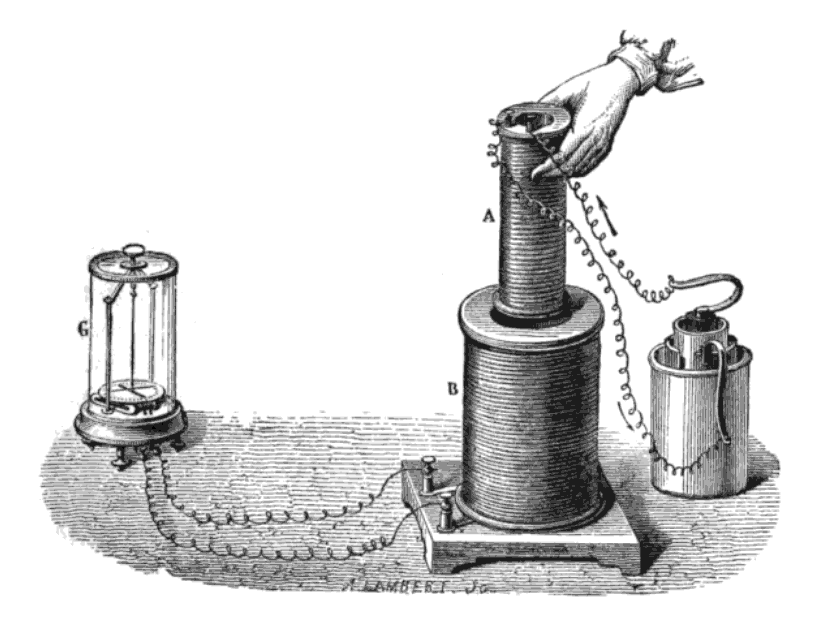
\includegraphics[width=0.53\textwidth]{./images/schematics/faraday_induction_experiment.png}\\
\end{center}

{\scriptsize
    The liquid battery (right) provides a current which flows through the small coil (A),
    creating a magnetic field. When the coils are stationary, no current is induced.
    But when the small coil is moved in or out of the large coil (B),
    the magnetic flux through the large coil changes,
    inducing a current which is detected by the galvanometer (G)
    [Wikipedia].\\
}

\end{frame}




%
%
%

\begin{frame}{Inductance}

We have seen the concepts of {\bf mutual} and {\bf self inductance}.\\

\vspace{0.2cm}

{\bf A change in current flow in a conductor induces a voltage (EMF)}
\begin{itemize}
   \item in the same conductor (self-inductance): \\
             $\displaystyle \mathcal{E} = - L \frac{dI}{dt}$
   \item and in neighbouring conductors (mutual inductance):\\
            $\displaystyle \mathcal{E}_{neighbouring\;loop} = - M \frac{dI}{dt}$
\end{itemize}

\vspace{0.2cm}

In both cases the inductance (mutual or self) is the {\bf constant of proportionality}
between the EMF developed and the rate of current change.

\vspace{0.2cm}

Inductance, like capacitance, is an {\bf intrinsically positive quantity}.

\end{frame}

%
%
%

%
%\begin{frame}{Inductance: An application from everyday life}
%
%Induction cooking heats a cooking vessel by magnetic induction,
%instead of by thermal conduction from a flame, or an electrical heating element.
%
%\vspace{0.2cm}
%
%\begin{columns}
%  \begin{column}{0.58\textwidth}
%    \begin{center}
%        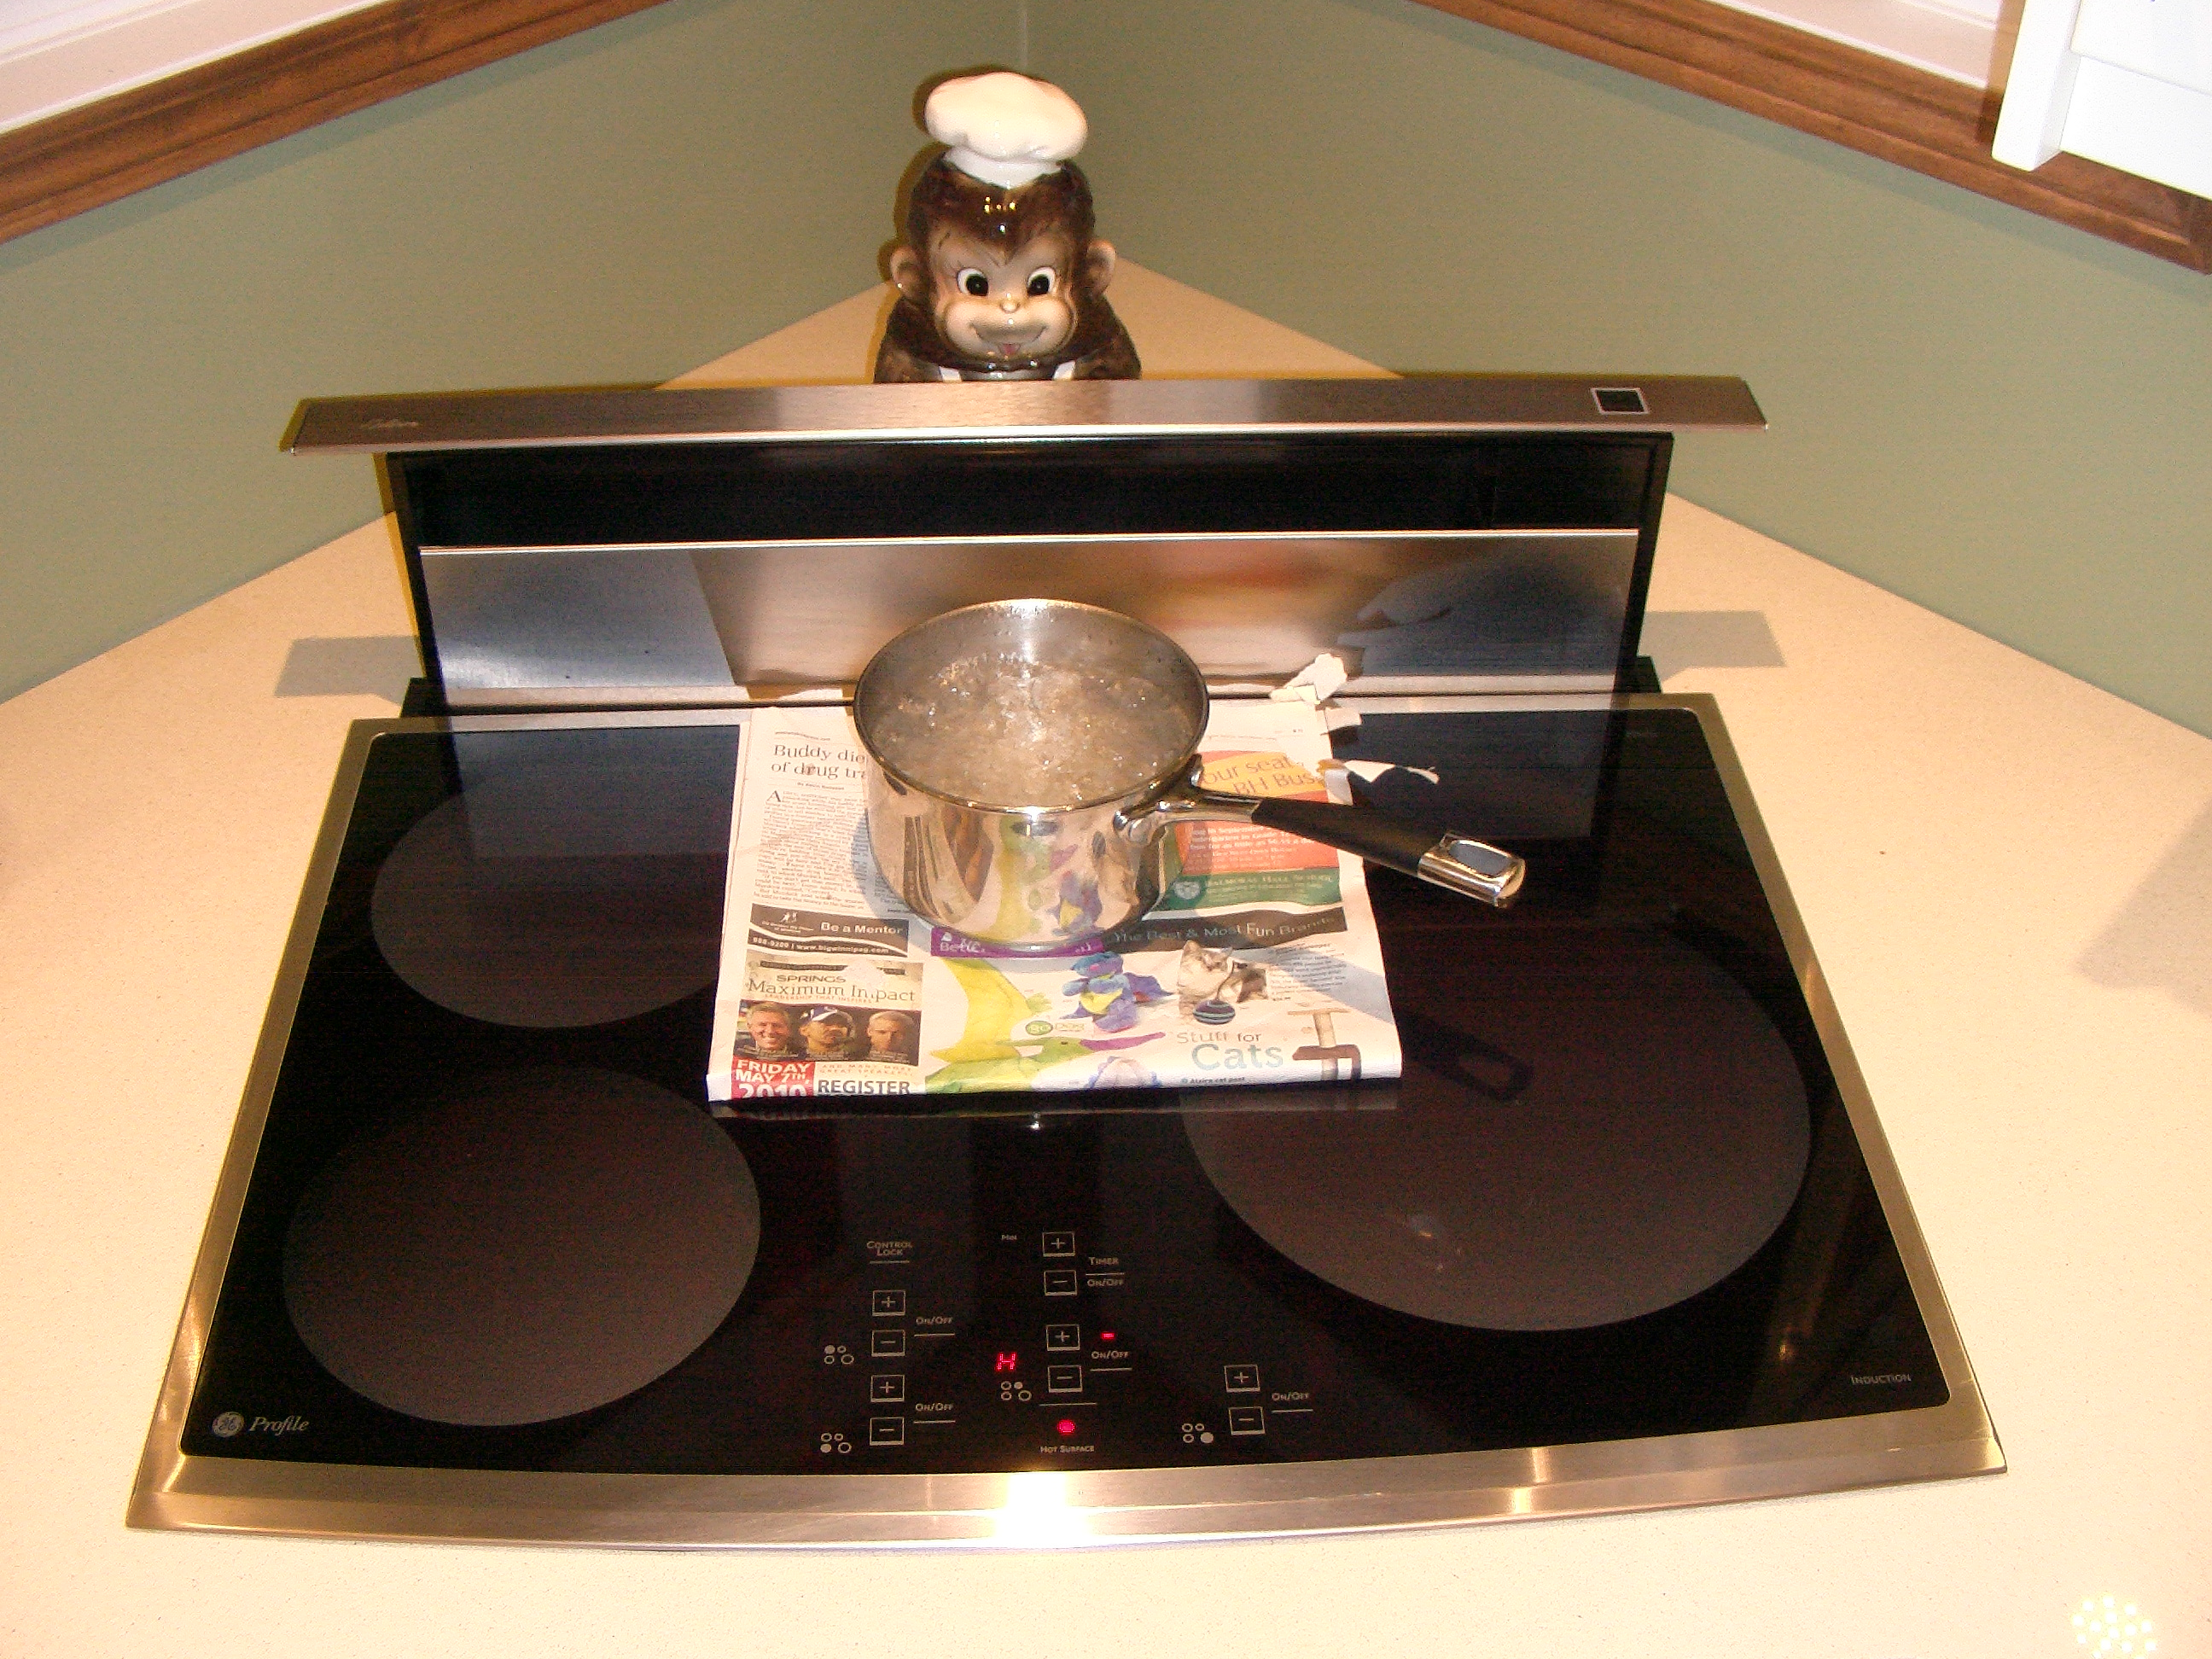
\includegraphics[width=0.98\textwidth]{./images/photos/induction_cooktop_rolling_boil.jpg}\\
%    \end{center}
%  \end{column}
%  \begin{column}{0.42\textwidth}
%  {\small
%    In an induction cooker, a coil of copper wire is placed under the cooking pot and an alternating
%    electric current is passed through it. The resulting oscillating magnetic field induces a magnetic flux
%    which repeatedly magnetises the pot, treating it like the lossy magnetic core of a transformer.
%    This produces large eddy currents in the pot, which because of the resistance of the pot, heats it
%    [Wikipedia].
%  }
%  \end{column}
%\end{columns}
%
%\end{frame}
%

%
%
%

\begin{frame}{Inductance: An application from everyday life}

{\bf Inductive wireless charging!}

\vspace{0.3cm}

\begin{columns}
  \begin{column}{0.50\textwidth}
    \begin{center}
        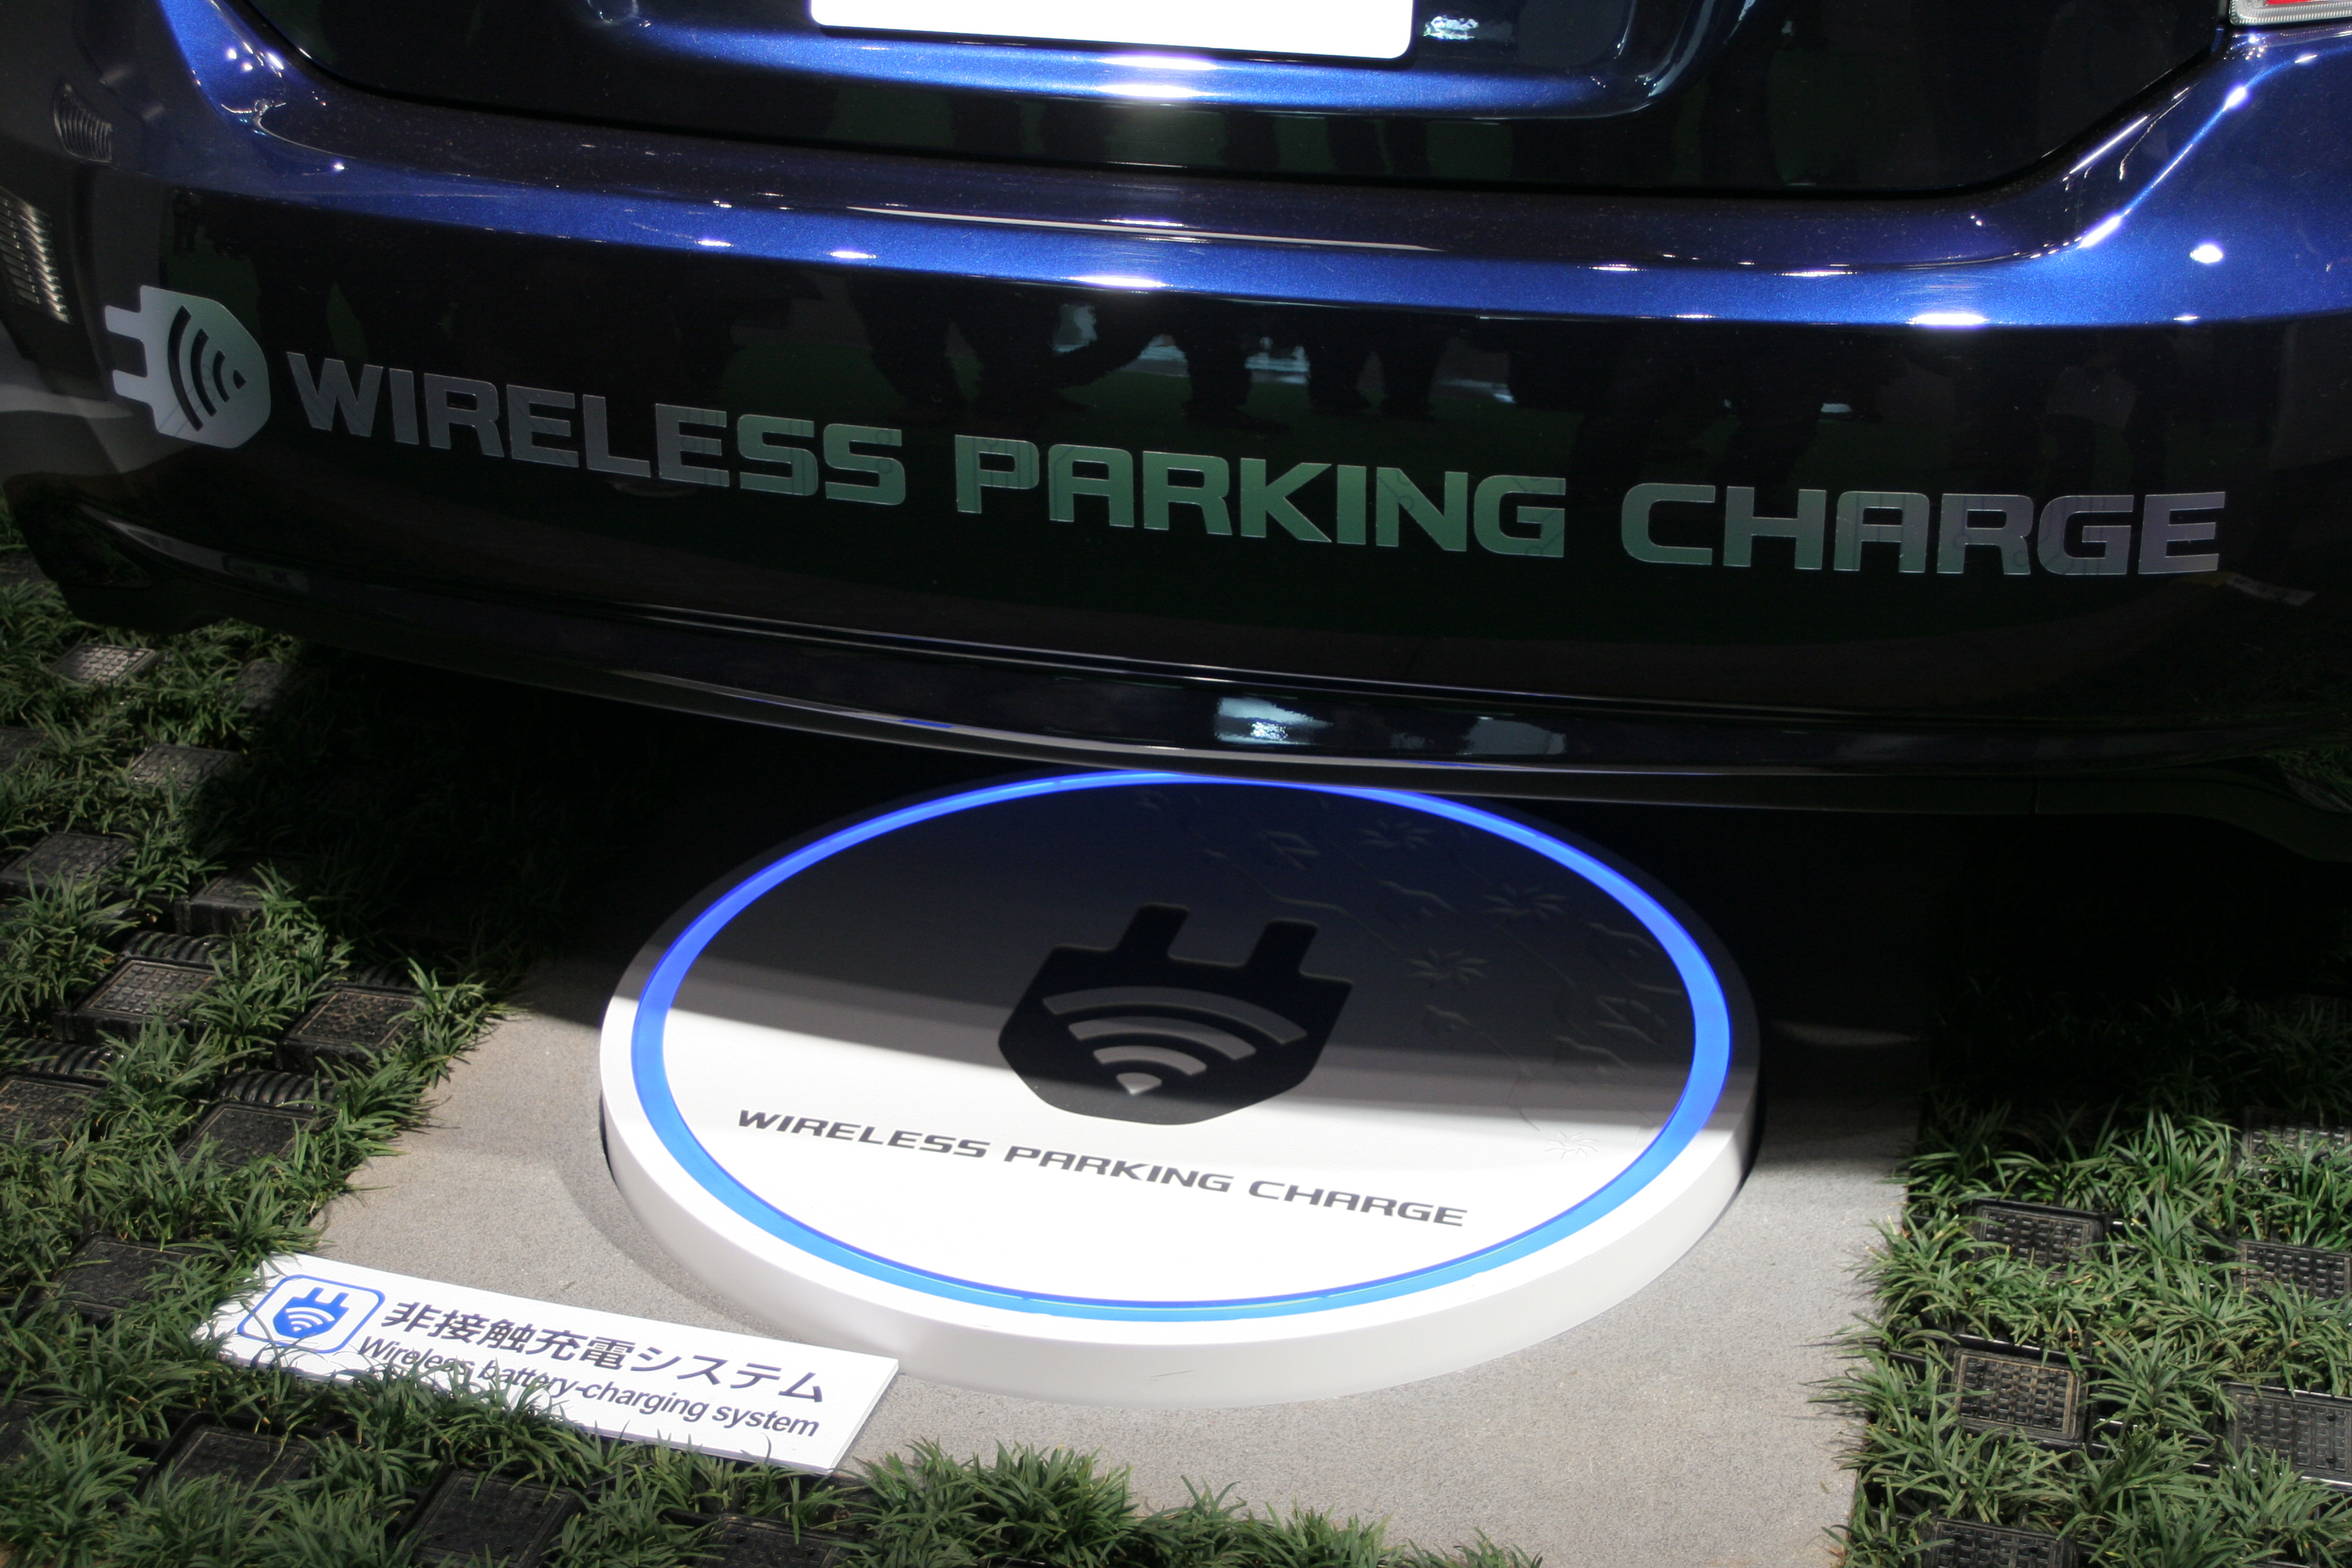
\includegraphics[width=0.98\textwidth]{./images/photos/electric_car_wireless_parking_charge_closeup.jpg}\\
     \end{center}
  \end{column}
  \begin{column}{0.50\textwidth}
    \begin{center}
        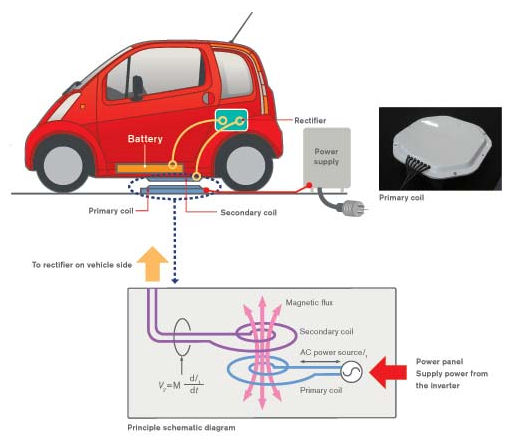
\includegraphics[width=0.98\textwidth]{./images/schematics/non_contact_charging.png}\\
     \end{center}
  \end{column}
\end{columns}

\end{frame}

%
%
%

\begin{frame}{Inductance: An application from everyday life}

{\bf Inductive wireless charging!}

\vspace{0.1cm}

\begin{center}
  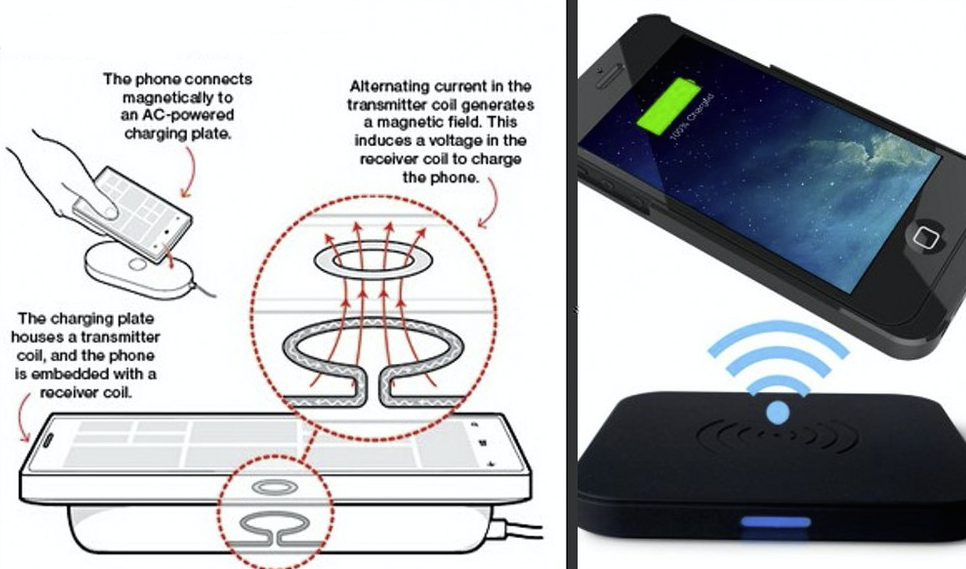
\includegraphics[width=0.90\textwidth]{./images/photos/inductive_charging_phone.png}\\
\end{center}

\end{frame}

%
%
%

\begin{frame}{Inductors and inductance}

An inductor is an electrical component which {\bf resists changes in electric current passing through it}.\\
\vspace{0.3cm}
An inductor is {\bf characterized by its inductance}
\begin{itemize}
   \item Typical values in the $\mu$H to H range.
\end{itemize}
\vspace{0.3cm}
It typically consists of a conductor such as a wire wound into a coil.\\
\vspace{0.3cm}
\begin{center}
  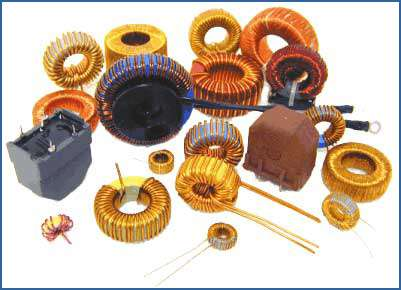
\includegraphics[width=0.45\textwidth]{./images/photos/inductors.jpg}\\
\end{center}

\end{frame}

%
%
%

\begin{frame}{Solenoids}

A solenoid is a coil wound into a tightly packed helix,
and whose length is substantially greater than its diameter.\\
\begin{itemize}
{\small
   \item Often wrapped around a metallic core which produces a uniform magnetic field.
}
\end{itemize}

\begin{center}
  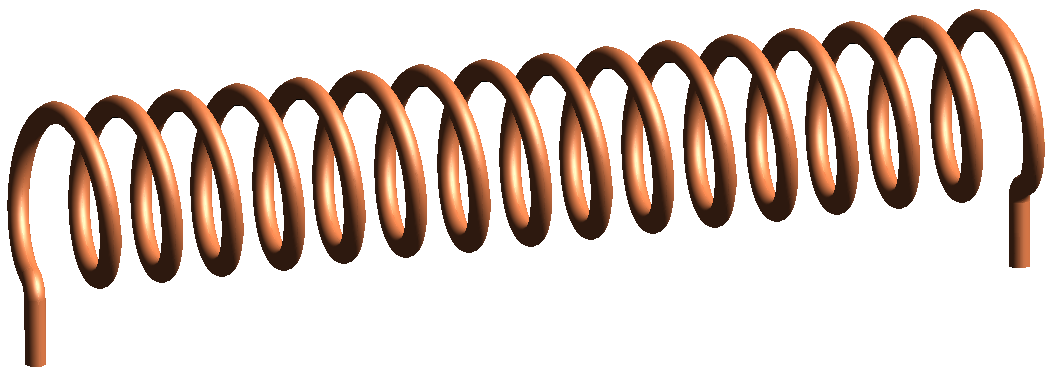
\includegraphics[width=0.40\textwidth]{./images/schematics/solenoid_1.png}\\
\end{center}

In a previous lecture we calculated the magnetic field produced
by a solenoid within its volume:
\begin{equation*}
   B = \mu_0 \cdot n \cdot I
\end{equation*}
where n is the number of windings per unit length and I is the current flowing in the coil.

\end{frame}

%
%
%

\begin{frame}{Inductance of solenoid}

If a current I produces a magnetic flux $\Phi_B$ in a loop, the inductance is defined to be:
\begin{equation*}
  L = \frac{\Phi_B}{I}
\end{equation*}

If the inductor is a coil made of N loops:
\begin{equation*}
  L = \frac{N \cdot \Phi_B}{I}
\end{equation*}

All the windings are linked by the shared flux $\Phi_B$.
The product $N \cdot \Phi_B$ is called the {\bf magnetic flux linkage}.

\end{frame}

%
%
%

\begin{frame}{Inductance of solenoid}

Consider a solenoid with n turns per unit length and area A.\\
\vspace{0.2cm}

The magnetic field is:
\begin{equation*}
    B = \mu_0 \cdot n \cdot  I
\end{equation*}

Over length x (away from its ends) the magnetic flux linkage is:
\begin{equation*}
    N \cdot \Phi_B = \Big( n \cdot  x \Big) \cdot \Big( B \cdot A \Big)
\end{equation*}

Hence:
\begin{equation*}
  L =
      \frac{N \cdot \Phi_B}{I} =
      \frac{\Big( n \cdot  x \Big) \cdot \Big( B \cdot A \Big)}{I} =
      \frac{\Big( n \cdot  x \Big) \cdot \Big( (\mu_0 \cdot n \cdot  I) \cdot A \Big)}{I} =
      \mu_0 \cdot n^2 \cdot x \cdot A
\end{equation*}

The inductance per unit length (far from the ends of the solenoid) is:
\begin{equation*}
{\color{magenta}
  L =  \mu_0 \cdot n^2 \cdot A
}
\end{equation*}

\end{frame}

%
%
%

\begin{frame}{Inductance in a circuit}

Now we will study the behaviour of electrical circuits which contain an element with inductance L
and, in particular, we will study
\begin{itemize}
  \item RL circuits,
  \item LC circuits and
  \item RLC circuits
\end{itemize}

\vspace{0.3cm}

An inductor is represented in circuit diagrams with the following symbol:
\begin{center}
  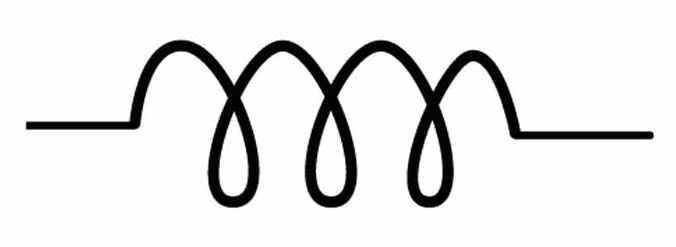
\includegraphics[width=0.25\textwidth]{./images/schematics/inductance_circuit_symbol.png}\\
\end{center}

\vspace{0.3cm}

The thing to remember is that, if there is a change in the current flowing through the inductor,
there will be a voltage developed across the conductor (back EMF) which is given by:
\begin{equation*}
    V_{L} =  -L \frac{dI}{dt}
\end{equation*}

\end{frame}

%
%
%

\begin{frame}{A simple circuit}

First, let’s examine a very simple DC circuit with an EMF and a resistor.\\
\vspace{0.4cm}

\begin{columns}
  \begin{column}{0.50\textwidth}
    \begin{center}
         \begin{circuitikz}
            \draw
                 (0,0) to[battery=$\varepsilon$] (0,2)
                         to[short, -o] (0.75, 2.0);
             \draw[very thick]
                  (0.78,2.0)--(1.22,2.0);
             \draw
                  (1.25, 2.0) to [short, o-] (2,2)
                                   to[R=$R$, i=$I$] (2,0) -- (0,0);
         \end{circuitikz}
     \end{center}
  \end{column}
  \begin{column}{0.50\textwidth}
        Kirchoff's voltage rule (the sum of EMFs in a closed loop equals the sum of potential drops):
       \begin{equation*}
         \sum_{i} \mathcal{E}_i = \sum_{j} I_{j} \cdot R_{j}
      \end{equation*}
  \end{column}
\end{columns}

\vspace{0.4cm}

Applying Kirchoff's voltage rule for the above circuit we get:
\begin{equation*}
          \mathcal{E} = I \cdot R \Rightarrow I = \frac{\mathcal{E}}{R}
\end{equation*}

\end{frame}


%
%
%

\begin{frame}{A simple circuit}

\begin{columns}
  \begin{column}{0.50\textwidth}
    Connecting the EMF:
    The current I takes {\bf instantaneously} the value $\mathcal{E}/R$ and remains constant.
    \begin{center}
         \begin{circuitikz}
            \draw
                 (0,0) to[battery=$\varepsilon$] (0,2)
                         to[short, -o] (0.75, 2.0);
             \draw[very thick]
                  (0.78,2.0)--(1.22,2.0);
             \draw
                  (1.25, 2.0) to [short, o-] (2,2)
                                   to[R=$R$, i=$I$] (2,0) -- (0,0);
             \draw
                  (1.25, 0) to [short, -o] (1.25,1.56);
         \end{circuitikz}
     \end{center}
     Disconnecting the EMF: the current stops (I=0) instananeously.
    \begin{center}
         \begin{circuitikz}
            \draw
                 (0,0) to[battery=$\varepsilon$] (0,2)
                         to[short, -o] (0.75, 2.0);
             \draw[very thick]
                  (1.25,1.59)--(1.25,2.0);
             \draw
                  (1.25, 2.0) to [short, o-] (2,2)
                                   to[R=$R$] (2,0) -- (0,0);
             \draw
                  (1.25, 0) to [short, -o] (1.25,1.56);
         \end{circuitikz}
     \end{center}
  \end{column}
  \begin{column}{0.50\textwidth}
      \begin{center}
          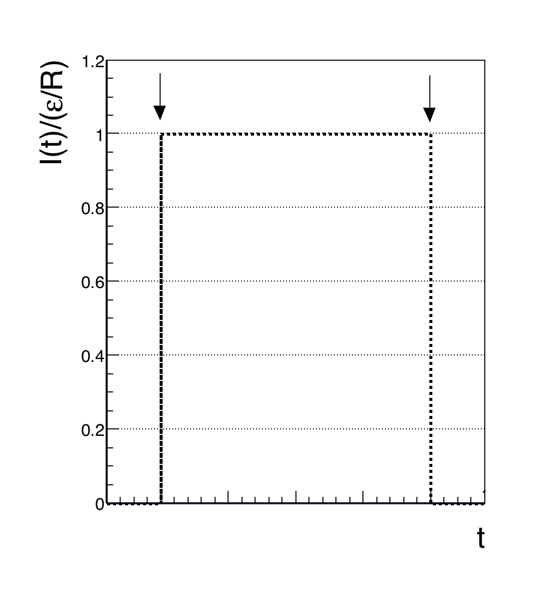
\includegraphics[width=0.96\textwidth]{./images/misc/ItR.png}\\
       \end{center}
  \end{column}
\end{columns}

\vspace{0.4cm}


\end{frame}

%
%
%

\begin{frame}{Adding inductance (The RL circuit)}

What happens if we {\bf add inductance in the circuit?}
Does your physics intuition tells you anything about the behaviour of the RL circuit?

\vspace{0.3cm}

\begin{columns}
  \begin{column}{0.60\textwidth}
   \begin{center}
         \begin{circuitikz} [scale=1.8]
            \draw
                 (0,0) to[battery=$\varepsilon$] (0,2)
                         to[short, -o] (0.75, 2.0);
             \draw[very thick]
                  (0.78,2.0)--(1.22,2.0);
             \draw
                  (1.25, 2.0) to [short, o-] (2,2)
                                   to[R=$R$, i=$I$] (2,0)
                                   to[L=$L$] (0,0);
         \end{circuitikz}
   \end{center}
  \end{column}
  \begin{column}{0.40\textwidth}
       {\bf Inductance is a kind of inertia in the circuit}. \\
      \vspace{0.2cm}
      So it is {\bf no longer possible to just change the current instantaneously}.
  \end{column}
\end{columns}

\end{frame}

%
%
%

\begin{frame}{RL circuit analysis}

Let's study the RL circuit more quantitatively.\\
\vspace{0.2cm}

\begin{columns}
  \begin{column}{0.40\textwidth}
    \begin{center}

         \begin{circuitikz}
            \draw
                 (0,0) to[battery=$\varepsilon$] (0,2)
                         to[short, -o] (0.75, 2.0);
             \draw[very thick]
                  (0.78,2.0)--(1.22,2.0);
             \draw
                  (1.25, 2.0) to [short, o-] (2,2)
                                   to[R=$R$, i=$I$] (2,0)
                                   to[L=$L$] (0,0);
         \end{circuitikz}

     \end{center}
  \end{column}
  \begin{column}{0.60\textwidth}
       Using Kirchoff’s voltage rule (the sum of EMFs in a closed loop equals the sum of potential drops):
       \begin{equation*}
         \sum_{i} \mathcal{E}_i = \sum_{j} I_{j} \cdot R_{j}
      \end{equation*}
  \end{column}
\end{columns}

This time I have to include the back-EMF ($\displaystyle -L\frac{dI}{dt}$), therefore:
\begin{equation*}
          \mathcal{E} -L \cdot \frac{dI}{dt} = I \cdot R
\end{equation*}

To figure out what the current $I$ is as a function of time, we need to solve this first
order differential equation above. Luckily, this is easy!

\end{frame}

%
%
%

\begin{frame}{RL circuit analysis}

\begin{equation*}
     \mathcal{E} -L \cdot \frac{dI}{dt} = I \cdot R \Rightarrow
     L \cdot \frac{dI}{dt} =  \mathcal{E} - I \cdot R \Rightarrow
     L \cdot \frac{dI}{\mathcal{E} - I \cdot R} =  dt \Rightarrow
\end{equation*}

\begin{equation*}
     L \cdot \int \frac{dI}{\mathcal{E} - I \cdot R} = \int  dt \Rightarrow
    -\frac{L}{R} \cdot \int \frac{d\Big( \mathcal{E} - I \cdot R \Big)}{\mathcal{E} - I \cdot R} = \int  dt \Rightarrow
\end{equation*}

\begin{equation*}
    -\frac{L}{R} \cdot ln\Big( \mathcal{E} - I \cdot R \Big) = t + {\color{blue}const } \Rightarrow
    ln\Big( \mathcal{E} - I \cdot R \Big) = - \frac{R}{L} t + {\color{blue} const^{\prime} } \Rightarrow
\end{equation*}

\begin{equation*}
    \mathcal{E} - I \cdot R = {\color{blue} const^{\prime \prime} }  \cdot exp^{-\frac{R}{L} t} \Rightarrow
\end{equation*}

\begin{equation*}
    {\color{magenta} I(t) = \frac{\mathcal{E}}{R} + {\color{blue} I_0 } \cdot exp^{-\frac{R}{L} t} }
\end{equation*}

where $I_0$ a constant defined by the initial conditions.

\end{frame}

%
%
%

\begin{frame}{RL circuit analysis}

We have the following solution to the $\displaystyle \mathcal{E} -L \cdot \frac{dI}{dt} = I \cdot R$ differential equation:
\begin{equation*}
    {\color{magenta} I(t) = \frac{\mathcal{E}}{R} + {\color{blue} I_0 } \cdot exp^{-\frac{R}{L} t} }
\end{equation*}

{\bf Initial condition}:\\
\begin{equation*}
       I(t=0) = 0 \Rightarrow  \frac{\mathcal{E}}{R} + {\color{blue} I_0 } = 0 \Rightarrow {\color{blue} I_0 } = - \frac{\mathcal{E}}{R}
\end{equation*}

Therefore, the solution to the above differential equation  can be written as:
\begin{equation*}
   I(t) = \frac{\mathcal{E}}{R} \Big(1 - exp^{-\frac{R}{L} t} \Big)
  \Rightarrow
   {\color{magenta}
       I(t) = \frac{\mathcal{E}}{R} \Big(1 - exp^{-\frac{t}{\tau}} \Big)
   }
\end{equation*}
where $\tau = L/R$ is a {\bf characteristic time constant for the RL circuit}.

\end{frame}

%
%
%

\begin{frame}{RL circuit analysis}

\begin{columns}
  \begin{column}{0.70\textwidth}
       \begin{center}
           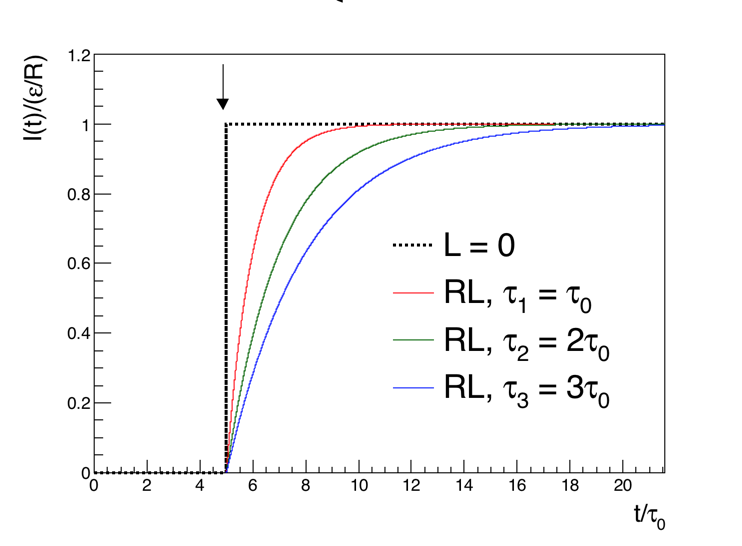
\includegraphics[width=0.95\textwidth]{./images/misc/ItRL_1.png}\\
       \end{center}
  \end{column}
  \begin{column}{0.30\textwidth}
      \begin{equation*}
       {\color{magenta}
            I(t) = \frac{\mathcal{E}}{R} \Big(1 - exp^{-\frac{t}{\tau}} \Big)
       }
      \end{equation*}
  \end{column}
\end{columns}

\end{frame}

%
%
%

\begin{frame}{RL circuit analysis}

{\bf What happens if I disconnect the EMF?}\\
{\small
The answer should be obvious by now. The current I will stop flowing, but the inertial effect
of inductance will prevent that from happening instantaneously. We expect the current to drop exponentially
towards zero.\\
}
\vspace{0.2cm}

\begin{columns}
  \begin{column}{0.40\textwidth}
    \begin{center}
         \begin{circuitikz} [scale=0.8]
            \draw
                 (0,0)--(0,2)--(2,2)
                        to[R=$R$, i=$I$] (2,0)
                        to[L=$L$] (0,0);
         \end{circuitikz}

     \end{center}
  \end{column}
  \begin{column}{0.60\textwidth}
       Once again, I need to start from Kirchhoff’s voltage rule. It gives me:
       \begin{equation*}
             -L \cdot \frac{dI}{dt} = I \cdot R
      \end{equation*}
  \end{column}
\end{columns}

Again, we need to solve the first order differential equation above to determine I(t).
Using the ssame procedure as before, and applying the asymptotic condition $I(t \rightarrow \infty) = 0$,
we get:
\begin{equation*}
{\color{magenta}
   I(t) = \frac{\mathcal{E}}{R} \cdot exp^{-\frac{t}{\tau}}
}
\end{equation*}
where $\tau = L/R$ is a {\bf characteristic time constant for the RL circuit}.

\end{frame}


%
%
%

\begin{frame}{RL circuit analysis}

\begin{columns}
  \begin{column}{0.70\textwidth}
       \begin{center}
           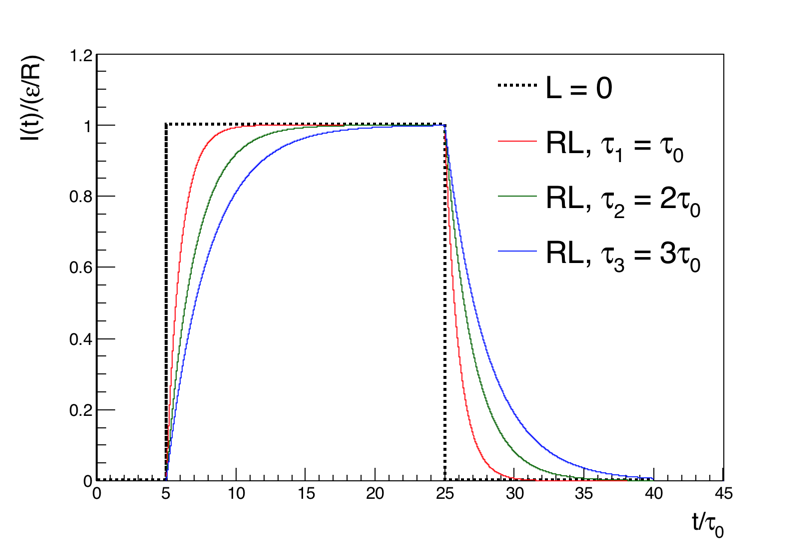
\includegraphics[width=0.95\textwidth]{./images/misc/ItRL_2.png}\\
       \end{center}
  \end{column}
  \begin{column}{0.30\textwidth}

      \begin{equation*}
       {\color{magenta}
            I(t) = \frac{\mathcal{E}}{R} \Big(1 - exp^{-\frac{t}{\tau}} \Big)
       }
      \end{equation*}

      \begin{equation*}
      {\color{magenta}
           I(t) = \frac{\mathcal{E}}{R} \cdot exp^{-\frac{t}{\tau}}
      }
      \end{equation*}

  \end{column}
\end{columns}

{\scriptsize
   Note that times are measured from the corresponding point of
   connecting or disconnecting the EMF.\\
}

\end{frame}

%
%
%

\begin{frame}{Energy stored in the magnetic field of an inductor}

Energy is stored in the magnetic field $\vec{B}$:
$\displaystyle U_B =\frac{1}{2\mu_0} \int_{\tau} d\tau |\vec{B}|^2$.\\
\vspace{0.1cm}

\begin{columns}
  \begin{column}{0.40\textwidth}
    \begin{center}

         \begin{circuitikz}
            \draw
                 (0,0) to[battery=$\varepsilon$] (0,2)
                         to[short, -o] (0.75, 2.0);
             \draw[very thick]
                  (0.78,2.0)--(1.22,2.0);
             \draw
                  (1.25, 2.0) to [short, o-] (2,2)
                                   to[R=$R$, i=$I$] (2,0)
                                   to[L=$L$] (0,0);
         \end{circuitikz}

     \end{center}
  \end{column}
  \begin{column}{0.60\textwidth}
       The differential equation describing the RL circuit was:
       \begin{equation*}
          \mathcal{E} = L \cdot \frac{dI}{dt} + I \cdot R
       \end{equation*}
  \end{column}
\end{columns}

Multiplying each side by I we have:
\begin{equation*}
{\color{magenta}
  \mathcal{E} \cdot I = L \cdot I \cdot \frac{dI}{dt} + I^2 \cdot R
}
\end{equation*}

As you know:
\begin{itemize}
{\small
   \item {\color{magenta} $\mathcal{E} \cdot I$ }
             is the rate at which energy is provided by the EMF source, and
   \item {\color{magenta} $I^2 \cdot R$ }
             is the rate at which energy is dissipated in the resistor.
}
\end{itemize}

\end{frame}

%
%
%

\begin{frame}{Energy stored in the magnetic field of an inductor}

\begin{equation*}
  \mathcal{E} \cdot I = {\color{magenta} L \cdot I \cdot \frac{dI}{dt} } + I^2 \cdot R
\end{equation*}

\begin{center}
   (rate at which energy is provided by the EMF source) = \\
      ? + (rate at which energy is dissipated in the resistor)
\end{center}

Therefore, the remaining term must describe the rate $\displaystyle \frac{dU_B}{dt}$
at which energy is stored in the magnetic field

\begin{equation*}
  \frac{dU_B}{dt} = L \cdot I \cdot \frac{dI}{dt} \Rightarrow
  \int dU_B = L \cdot \int I \cdot dI \Rightarrow
   U_B = \frac{1}{2} L \cdot I^2 + const
\end{equation*}

\vspace{0.2cm}
$U_B$=0 if I=0, hence:
\begin{equation*}
{\color{magenta}
   U_B = \frac{1}{2} L \cdot I^2
}
\end{equation*}

\end{frame}

%
%
%

\begin{frame}{Energy stored in the magnetic field of an inductor}

{\it A sanity check}:\\

\vspace{0.3cm}

Consider the solenoid studied earlier in this lecture. Assume a solenoid with length x,
cross-sectional area A and n turns per unit length.\\

\vspace{0.2cm}

The magnetic energy stored in the solenoid is:
\begin{equation*}
  U_B = \frac{1}{2} L I^2 \xRightarrow{\frac{L}{x} = \mu_0 n^2 A}
  U_B = \frac{1}{2} \mu_0 (Ax) n^2 I^2
\end{equation*}
The magnetic energy per unit volume is:
\begin{equation*}
  u_B = \frac{U_B}{Ax} = \frac{\frac{1}{2} \mu_0 (Ax) n^2 I^2}{Ax} =
           \frac{1}{2} \mu_0 n^2 I^2 \xRightarrow{B = \mu_0 n I}
  u_B = \frac{B^2}{2\mu_0}
\end{equation*}

as expected!

\end{frame}

%
%
%

\begin{frame}{LC electrical circuits}

Now, we are going to examine the so-called {\bf LC electrical circuits}
that consist of an inductor L and a capacitor C.
\begin{itemize}
    \item LC circuits are also called {\bf resonant circuits} for reasons
              that will become clear in the next lecture.
\end{itemize}

Let’s assume that at some initial time, the {\bf capacitor is fully charged} and
then it is left to discharge via the inductor.

Here is a simple representation of such a circuit.

\begin{center}

         \begin{circuitikz} [scale=1.5]
            \draw
                 (0,0) to[battery=$\varepsilon$] (0,2) to[short, -o] (0.75, 2.0);
             \draw[very thick]
                  (0.78,2.0)--(1.18,2.3);
             \draw
                  (1.25, 2.0) to [short, o-] (2,2) to[C=$C$] (2,0)--(0,0);
              \draw
                  (2,2)--(4,2) to[L=$L$,i=$I$] (4,0) -- (2,0);
         \end{circuitikz}

\end{center}

\end{frame}

%
%
%

\begin{frame}{LC electrical circuits}

The {\bf capacitor stores energy in the electric field} between its plates.\\

\vspace{0.2cm}
As we have seen the energy stored in a charged capacitor is:
\begin{equation*}
  U_E = \frac{1}{2}CV^2
\end{equation*}

The capacitor is connected to an inductor and it is discharged.\\

\vspace{0.2cm}

The current flowing will {\bf build up a magnetic field in the inductor}.\\

\vspace{0.2cm}

The {\bf inductor stores energy in its magnetic field}.\\

\vspace{0.2cm}

As we have seen the energy stored in an inductor is:
\begin{equation*}
  U_B = \frac{1}{2}LI^2
\end{equation*}

\end{frame}


%
%
%

\begin{frame}{LC electrical circuits}

\begin{itemize}
\item
  At some initial time, the {\bf capacitor is fully charged} so {\bf all energy is stored in the electric field}.\\
\item
  As it is discharged, the current builds up the the magnetic field in the inductor so the {\bf energy is
  transferred from the electric to magnetic field}.
\item
  Once the {\bf capacitor is fully discharged, all energy is stored in the magnetic field.}
  \vspace{0.3cm}
\item
  Even though the capacitor is now fully discharged the current will continue because
  inductors resist changes in the current.
\item
   The current will start charging up the capacitor again, but with a voltage of opposite polarity.
\item
   So energy starts moving back again from the magnetic field to the newly re-created electric
  field of the capacitor!
\end{itemize}

\end{frame}



%
%
%

\begin{frame}{LC electrical circuits}

\begin{center}
  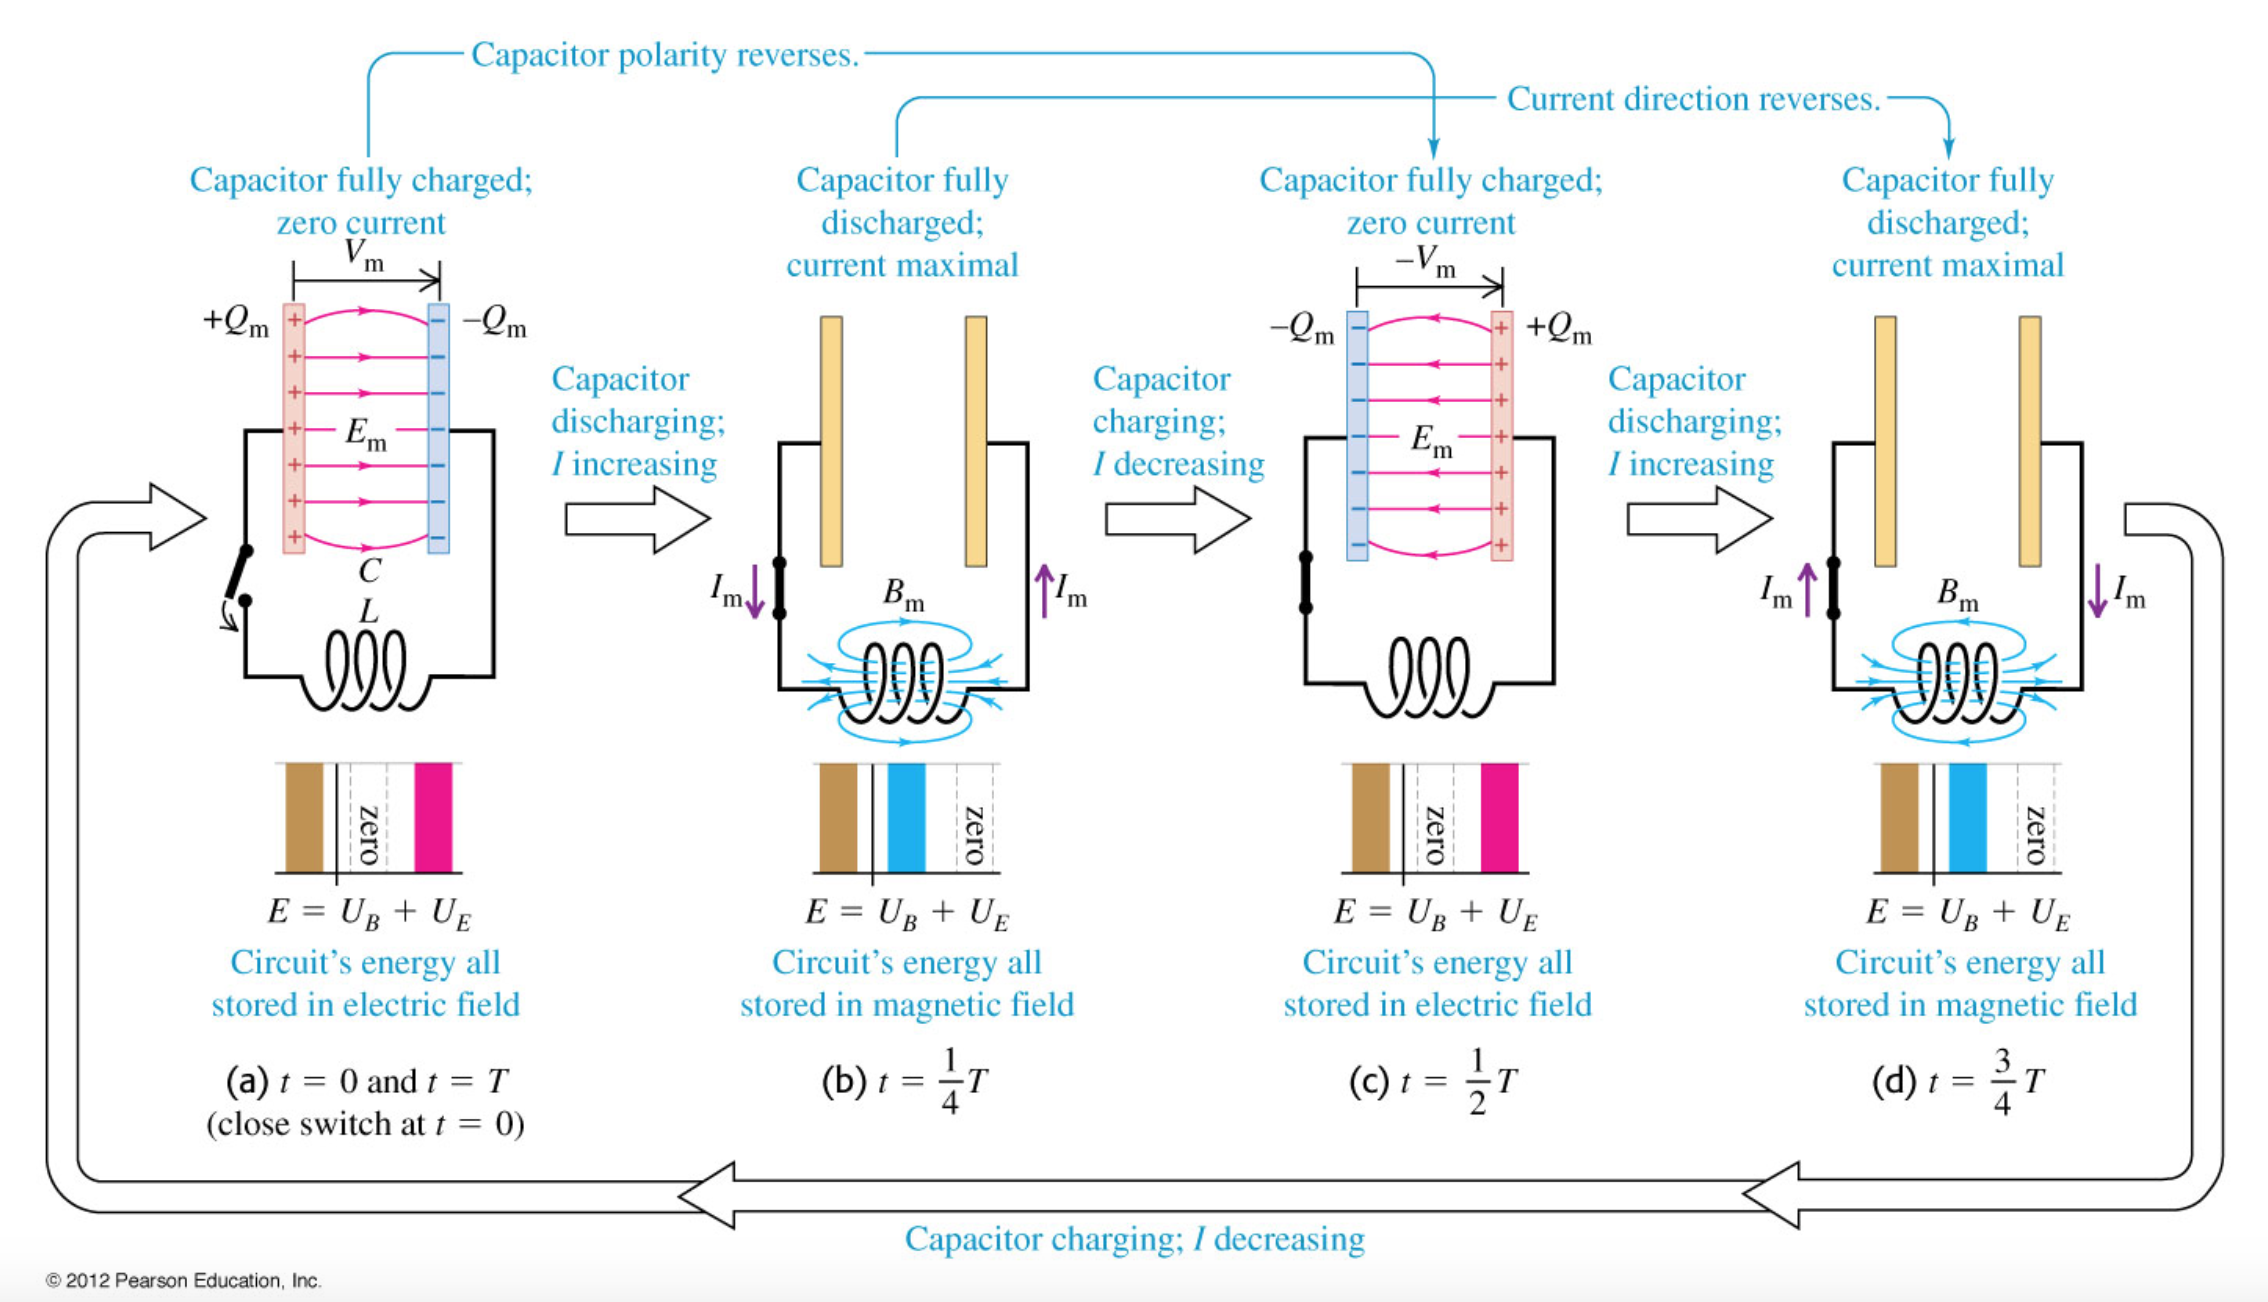
\includegraphics[width=0.99\textwidth]{./images/schematics/LC_oscillations.png}\\
\end{center}

\end{frame}


%
%
%

\begin{frame}{LC electrical circuit analysis}

Let’s do a more quantitative analysis of what we described above:\\
\vspace{0.2cm}

\begin{columns}
  \begin{column}{0.40\textwidth}
    \begin{center}
         \begin{circuitikz}
              \draw
                  (0,0) to[C=$C$] (0,2)--(2,2) to[L=$L$,i=$I$] (2,0) -- (0,0);
         \end{circuitikz}
     \end{center}
  \end{column}
  \begin{column}{0.60\textwidth}
     Using Kirchhoff’s voltage rule:
     We take into account is the back-EMF because of the
     inductance and the voltage across the capacitor plates.
  \end{column}
\end{columns}

\vspace{0.5cm}

Therefore:
\begin{equation*}
      -L \frac{dI}{dt} = \frac{q}{C} \xRightarrow{I = \frac{dq}{dt}}
      -L \frac{d}{dt} \frac{dq}{dt} = \frac{q}{C} \Rightarrow
\end{equation*}

\begin{equation*}
  {\color{magenta}
       \frac{d^2q}{dt^2} + \frac{1}{LC} q = 0
  }
\end{equation*}

\end{frame}

%
%
%

\begin{frame}{LC electrical circuit analysis}

I am sure that you have seen a similar equation before as it is commonly derived in many
different physical settings.

\begin{equation*}
  {\color{magenta}
       \frac{d^2q}{dt^2} + \frac{1}{LC} q = 0
  }
\end{equation*}

{\bf Do you recognize it?}\\

\vspace{0.2cm}
This {\bf second order differential equation} is similar to the equation for a simple
harmonic oscillator, that is the equation for an oscillator that is neither driven nor damped.

\begin{center}
  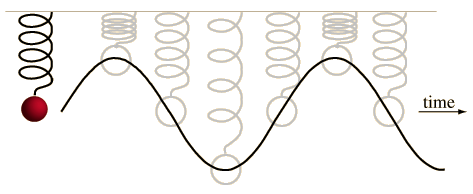
\includegraphics[width=0.50\textwidth]{./images/schematics/harmonic_oscillator.png}\\
\end{center}


\end{frame}

%
%
%

\begin{frame}{The harmonic oscillator equation}

For example, assume a mass m, which experiences a force F which pulls the mass towards x = 0.
\begin{equation*}
   F = -kx
\end{equation*}

Using Newton's 2$^{nd}$ law, we have:
\begin{equation*}
   F = m \frac{d^2x}{dt^2} = -kx \Rightarrow
   {\color{magenta}
       \frac{d^2x}{dt^2} + \frac{k}{m} x = 0
   }
\end{equation*}

The motion of the mass m is periodic and it is described by the function:
\begin{equation*}
   x(t) = x_0 cos\Big( \omega t + \phi \Big)
\end{equation*}
where $x_0$ is the constant amplitude of the periodic motion,
$\omega$ the angular frequency of the oscillation defined by
\begin{equation*}
   \omega = \sqrt{\frac{k}{m}} \Big( = \frac{2\pi}{T} \Big)
\end{equation*}
and $\phi$ is a phase determined by the initial conditions.

\end{frame}


%
%
%

\begin{frame}{An LC circuit executes simple harmonic oscillations}

Now contrast
\begin{equation*}
    \frac{d^2q}{dt^2} + \frac{1}{LC} q = 0
    \;\;\;\;\;\; with \;\;\;\;\;\;
    \frac{d^2x}{dt^2} + \frac{k}{m} x = 0
\end{equation*}

We can conclude that the {\bf charge q(t) in an LC circuit oscillates harmonically}:
\begin{equation*}
   q(t) = q_0 cos\Big( \omega t + \phi \Big)
\end{equation*}

where $q_0$ is the constant amplitude of the oscillation (the max quantity of
charge accumulated on the capacitor plates) and
$\omega$ the angular frequency of the oscillation defined by
\begin{equation*}
   \omega = \frac{1}{\sqrt{LC}}
\end{equation*}
As before, $\phi$ is a phase determined by the initial conditions.

\begin{equation*}
   I(t) = \frac{dq(t)}{dt} =
       \frac{d}{dt} \Big\{ q_0 cos\Big( \omega t + \phi \Big) \Big\} =
        - q_0 \omega sin\Big( \omega t + \phi \Big)
\end{equation*}

\end{frame}

%
%
%

\begin{frame}{Energy oscillations in an LC circuit}

{\bf The energy stored in the capacitor is}:
\begin{equation*}
  U_E(t)= \frac{1}{2} CV(t)^2 = \frac{1}{2} C \Big( \frac{q(t)}{C} \Big)^2 = \frac{1}{2C} q(t)^2
 \xRightarrow{q(t) = q_0 cos\Big( \omega t + \phi \Big)}
\end{equation*}
\begin{equation*}
  U_E(t) = \frac{1}{2C} \Big\{ q_0 cos\Big( \omega t + \phi \Big) \Big\}^2 \Rightarrow
  {\color{magenta}
      U_E(t) = \frac{q_0^2}{2C} cos^{2}\Big( \omega t + \phi \Big)
 }
\end{equation*}

\vspace{0.2cm}

{\bf The energy stored in the inductor is:}
\begin{equation*}
  U_B(t) = \frac{1}{2} LI(t)^2 \xRightarrow{ I(t) = - q_0 \omega sin\Big( \omega t + \phi \Big)}
  U_B(t) = \frac{1}{2} L \Big\{ - q_0 \omega sin\Big( \omega t + \phi \Big) \Big\}^2
\end{equation*}
\begin{equation*}
   U_B(t) = \frac{1}{2} L q_0^2 \omega^2 sin^2\Big( \omega t + \phi \Big) \xRightarrow{\omega = \frac{1}{\sqrt{LC}}}
\end{equation*}
\begin{equation*}
   U_B(t) = \frac{1}{2} L q_0^2 \frac{1}{LC} sin^2\Big( \omega t + \phi \Big)
  \Rightarrow
  {\color{magenta}
      U_B(t) = \frac{q_0^2}{2C} sin^2\Big( \omega t + \phi \Big)
  }
\end{equation*}

\end{frame}

%
%
%

\begin{frame}{Energy oscillations in LC an circuit}

So $U_E(t)$ and $U_B(t)$ oscillate!

\begin{equation*}
  {\color{magenta}
      U_E(t) = \frac{q_0^2}{2C} cos^{2}\Big( \omega t + \phi \Big)
 }
\end{equation*}

\begin{equation*}
  {\color{magenta}
      U_B(t) = \frac{q_0^2}{2C} sin^2\Big( \omega t + \phi \Big)
  }
\end{equation*}

Notice that:
\begin{itemize}
  \item $U_E(t)$ and $U_B(t)$ have the same amplitude $\displaystyle \frac{q_0^2}{2C}$
    \begin{itemize}
        \item The stored energy is fully transferred between the
                  electric and magnetic fields (i.e. between the capacitor and the inductor).
    \end{itemize}
  \item They have a phase difference of $pi/2$ ($cos^2x \rightarrow sin^2x$)
    \begin{itemize}
        \item The energy stored in the electric field at some particular time t,
                  is the same amount of energy stored in the magnetic field at t$^\prime$ = t + T/4
    \end{itemize}
\end{itemize}


\end{frame}

%
%
%

\begin{frame}{Energy oscillations in LC an circuit}

{\bf How about the total energy U(t)?}

\begin{equation*}
  U(t) = U_E(t) + U_B(t) \Rightarrow
\end{equation*}

\begin{equation*}
  U(t) = \frac{q_0^2}{2C} cos^{2}\Big( \omega t + \phi \Big) +
            \frac{q_0^2}{2C} sin^{2}\Big( \omega t + \phi \Big) \Rightarrow
\end{equation*}
\begin{equation*}
  U(t) = \frac{q_0^2}{2C} \Big\{ cos^{2}\Big( \omega t + \phi \Big) + sin^2\Big( \omega t + \phi \Big) \Big\} \Rightarrow
\end{equation*}
\begin{equation*}
{\color{magenta}
  U(t) = \frac{q_0^2}{2C}
}
\end{equation*}

{\bf The total energy stored is constant} (as it should!)\\
\begin{itemize}
    \item In the above system there was no mechanism for dissipating energy.
\end{itemize}

\end{frame}


%
%
%

\begin{frame}{Energy oscillations in LC circuit}

\begin{center}
     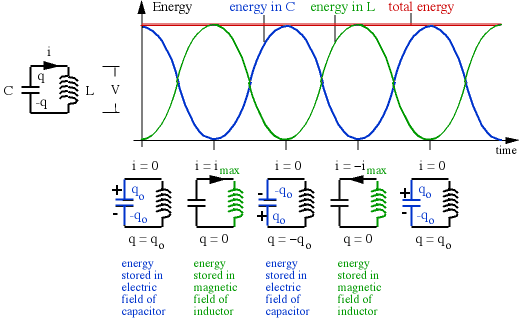
\includegraphics[width=0.95\textwidth]{./images/schematics/LC_oscillations_2.png}\\
\end{center}

\end{frame}

%
%
%

\begin{frame}{RLC electrical circuit}

In the LC circuit, the stored energy was {\bf fully transferred} between the
electric and magnetic fields (i.e. between the capacitor and the inductor).\\
\vspace{0.2cm}
In absence of a mechanism for dissipating energy, the
total energy stored in the LC circuit was constant.\\
\vspace{0.2cm}
Now, we will study a more realistic system: A system with capacitance (C),
inductance (L) and resistance (R).\\
\vspace{0.2cm}

\begin{center}
         \begin{circuitikz} [scale=1.5]
            \draw
                 (0,0) to[battery=$\varepsilon$] (0,2) to[short, -o] (0.75, 2.0);
             \draw[very thick]
                  (0.78,2.0)--(1.18,2.3);
             \draw
                  (1.25, 2.0) to [short, o-] (2,2) to[C=$C$] (2,0)--(0,0);
              \draw
                  (2,2) to[R=$R$]  (4,2) to[L=$L$,i=$I$] (4,0) -- (2,0);
         \end{circuitikz}
\end{center}

\end{frame}

%
%
%

\begin{frame}{RLC electrical circuit}

Based on what we discuss, we can guess the behaviour of the RLC circuit:

\begin{itemize}
  \item
    As with the LC circuit, the energy will oscillated between the electric field of the capacitor
    and the magnetic field of the inductor.
  \item
    But we also have a resistor in the circuit, so the energy will not be fully transferred
    between the electric and magnetic field.
  \item
    Indeed, with every cycle, a fraction of the available stored energy would be lost (transformed to heat).
\end{itemize}

\vspace{0.3cm}

So, again, we will have energy oscillations.\\

\vspace{0.3cm}

But, in this case, the oscillations will be {\bf damped}.\\

\end{frame}


%
%
%

\begin{frame}{RLC circuit analysis}

Let’s do a more quantitative analysis of what we described above:

\begin{columns}
  \begin{column}{0.40\textwidth}
    \begin{center}
         \begin{circuitikz} [scale=1.5]
             \draw
                  (0,0) to[C=$C$] (0,2) to[R=$R$]  (2,2) to[L=$L$,i=$I$] (2,0) -- (0,0);
         \end{circuitikz}
     \end{center}
  \end{column}
  \begin{column}{0.60\textwidth}
       Using Kirchoff's voltage rule:
       \begin{equation*}
          -L \frac{dI}{dt} = RI + \frac{q}{C} \xRightarrow{I = dq/dt}
       \end{equation*}
       \begin{equation*}
       {\color{magenta}
            L \frac{d^2q}{dt^2} + R \frac{dq}{dt} + \frac{1}{C}q = 0
       }
       \end{equation*}
  \end{column}
\end{columns}

\vspace{0.5cm}

To obtain q=q(t) we have to solve the 2$^{nd}$ order differential equation.

\vspace{0.2cm}

We will not do this here.

\end{frame}


%
%
%

\begin{frame}{RLC circuit analysis}

The differential equation:
\begin{equation*}
     L \frac{d^2q}{dt^2} + R \frac{dq}{dt} + \frac{1}{C}q = 0
\end{equation*}

has the following solution:
\begin{equation*}
{\color{magenta}
  q = q_0 e^{-\frac{R}{2L}t} cos\Big(\omega^{\prime} t + \phi \Big)
}
\end{equation*}

where
\begin{equation*}
   {\color{magenta}
       \omega^{\prime} = \sqrt{\omega^2 - \Big( \frac{R}{2L} \Big)^2}
    }
    \;\;\;\;\; and \;\;\;\;\;
    \omega = \frac{1}{\sqrt{LC}}
\end{equation*}

\vspace{0.2cm}

You should confirm (on your own)
that the above is indeed a solution of the differential equation.

\end{frame}

%
%
%

\begin{frame}{RLC circuit analysis}

Notice that the {\bf frequency of oscillation is now different}:
\begin{equation*}
   {\color{magenta}
       \omega \rightarrow \omega^{\prime} = \sqrt{\omega^2 - \Big( \frac{R}{2L} \Big)^2}
    }
    \;\;\;\;\; and \;\;\;\;\;
    \omega = \frac{1}{\sqrt{LC}}
\end{equation*}
If R = 0, then $ \omega^{\prime} =  \omega = \frac{1}{\sqrt{LC}}$ as expected.

\vspace{0.5cm}

But the most striking feature is that now the {\bf amplitude is not constant,
but it falls exponentially as time increases}.

\begin{equation*}
{\color{magenta}
    q_0  \rightarrow q_0 e^{-\frac{R}{2L}t}
}
\end{equation*}

{\bf The oscillation is damped}:
\begin{itemize}
  \item Energy not fully oscillating between the electric and magnetic field.
  \item In every period, an amount of energy is converted to heat by the resistor and it is lost.
\end{itemize}

\end{frame}


%
%
%

\begin{frame}{RLC circuit: Damped current oscillations}

% Consider a situation where $ \omega^{\prime} \approx  \omega$.
% \begin{itemize}
%    \item The damping is not too strong.
% \end{itemize}

% \vspace{0.3cm}

The current is given by:

\begin{equation*}
   I(t) = \frac{dq}{dt} = \frac{d}{dt}  \Big\{ q_0 e^{-\frac{R}{2L}t} cos\Big(\omega^{\prime} t + \phi \Big) \Big\} \Rightarrow
\end{equation*}

\begin{equation*}
   I(t) =  -\frac{R}{2L} q_0 e^{-\frac{R}{2L}t} cos\Big(\omega^{\prime} t + \phi \Big)
             -\omega^{\prime} q_0 e^{-\frac{R}{2L}t} sin\Big(\omega^{\prime} t + \phi \Big)
\end{equation*}

\begin{center}
     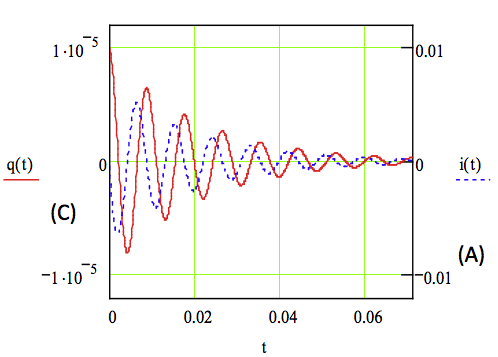
\includegraphics[width=0.50\textwidth]{./images/misc/ItRLC.png}\\
\end{center}

\end{frame}

%
%
%

\begin{frame}{RLC circuit: Damped energy oscillations}

\begin{equation*}
  U_E(t) = \frac{q^2}{2C} = \frac{q_0}{2C} e^{-\frac{R}{L}t} cos^{2}\Big(\omega^{\prime} t + \phi \Big)
\end{equation*}

\begin{equation*}
  U_B(t) = \frac{1}{2}LI^2 = \frac{1}{2}L
                 \Big\{
                     \frac{R}{2L} q_0 e^{-\frac{R}{2L}t} cos\Big(\omega^{\prime} t + \phi \Big) +
                     \omega^{\prime} q_0 e^{-\frac{R}{2L}t} sin\Big(\omega^{\prime} t + \phi \Big)
                  \Big\}^2
\end{equation*}

\begin{center}
     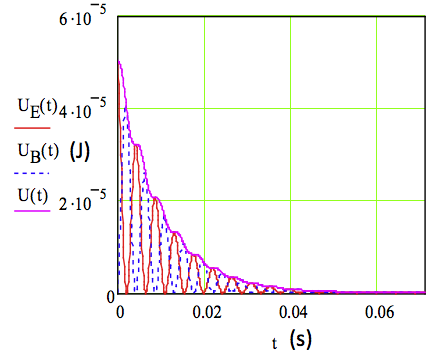
\includegraphics[width=0.50\textwidth]{./images/misc/UtRLC.png}\\
\end{center}

\end{frame}


% ------------------------------------------------------------------------------
% ------------------------------------------------------------------------------

%
% What to remember
%

\renewcommand{\lecturesummarytitle}{Main points to remember }

\renewcommand{\summarizedlecture}{11 }

%
%
%

\begin{frame}{Lecture \summarizedlecture - \lecturesummarytitle}

\begin{columns}
  \begin{column}{0.25\textwidth}
    \begin{center}
       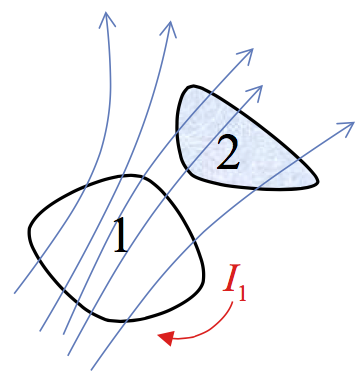
\includegraphics[width=0.90\textwidth]{./images/schematics/mutual_inductance_1.png}\\
     \end{center}
  \end{column}
  \begin{column}{0.75\textwidth}
  {\scriptsize
       The flux through the surface of loop 2, of the magnetic field $\vec{B}_1$
       produced by the current $I_1$ in loop 1 is:
       \begin{equation*}
            \Phi_2 = M_{21}  I_1
       \end{equation*}
       The constant of proportionality ($M_{21}$) is known as {\bf mutual inductance}.\\
       It is:
       \begin{itemize}
           \item purely geometrical, and
           \item unchanged if one switches the roles of loop 1 and 2.\\
       \end{itemize}
   }
  \end{column}
\end{columns}

\vspace{0.4cm}

{\scriptsize
       So \underline{whatever} the shapes and positions of the loops,
       the flux through loop 2 when we run a current I around loop 1 is
       identical to the flux through loop 1 when we run the same current around loop 2.
      \begin{equation*}
            M_{21}  = M_{12} = M
       \end{equation*}

        The SI unit of the mutual inductance is the {Henry} (H)
        \begin{itemize}
              \item A derived unit.
              \item 1 H = $\displaystyle \frac{Wb}{A}$ = $\displaystyle \frac{V \cdot s}{A}$
        \end{itemize}
}
\end{frame}

%
%
%

\begin{frame}{Lecture \summarizedlecture - \lecturesummarytitle (cont'd)}

{ \scriptsize
We also considered what happens if the current varies with time.
\begin{itemize}
  { \scriptsize
   \item  time-varying current $\rightarrow$ time-varying magnetic field
   \item  time-varying magnetic field $\rightarrow$  time-varying flux.
   \item  time-varying flux $\rightarrow$ EMF (Faraday's law)
  }
\end{itemize}

\vspace{0.3cm}

{\bf A change in current flow in a conductor induces a voltage (EMF)}
\vspace{0.2cm}
\begin{itemize}
  { \scriptsize
   \item in the same conductor (self-inductance): \\
             $\displaystyle \mathcal{E} = - L \frac{dI}{dt}$
   \vspace{0.2cm}
   \item and in neighbouring conductors (mutual inductance):\\
            $\displaystyle \mathcal{E}_{neighbouring\;loop} = - M \frac{dI}{dt}$
  }
\end{itemize}

\vspace{0.2cm}

In both cases the inductance (mutual or self) is the {\bf constant of proportionality}
between the EMF developed and the rate of current change.

\vspace{0.2cm}

We also studied the solenoid and its inductance per unit length (far from the ends of the solenoid) is:
\begin{equation*}
  L =  \mu_0 \cdot n^2 \cdot A
\end{equation*}
where $A$ is the area of each winding, and $n$ the number of turns per unit length.
}
\end{frame}

%
%
%

\begin{frame}{Lecture \summarizedlecture - \lecturesummarytitle (cont'd)}

Then we studied DC circuits with resistors, capacitors and inductors.

\begin{columns}
  \begin{column}{0.40\textwidth}
    \begin{center}
         \begin{circuitikz} [scale=0.7]
            \draw
                 (0,0) to[battery=$\varepsilon$] (0,2)
                         to[short, -o] (0.75, 2.0);
             \draw[very thick]
                  (0.78,2.0)--(1.22,2.0);
             \draw
                  (1.25, 2.0) to [short, o-] (2,2)
                                   to[R=$R$, i=$I$] (2,0)
                                   to[L=$L$] (0,0);
         \end{circuitikz}
     \end{center}
  \end{column}
  \begin{column}{0.60\textwidth}
   {\scriptsize
       We studied an RL circuit and we saw that its behaviour is determined
      by the following differential equation:
       \begin{equation*}
              \mathcal{E} -L \cdot \frac{dI}{dt} = I \cdot R
      \end{equation*}
   }
  \end{column}
\end{columns}

\begin{columns}
  \begin{column}{0.40\textwidth}
       \begin{center}
           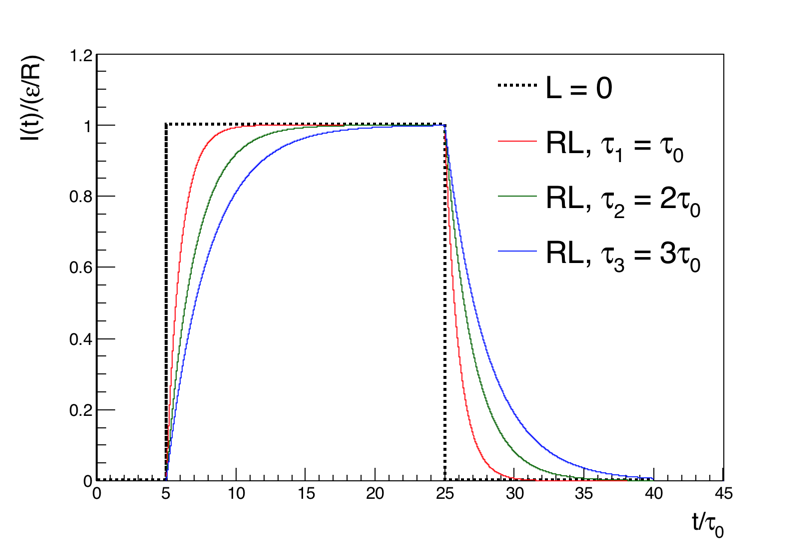
\includegraphics[width=0.95\textwidth]{./images/misc/ItRL_2.png}\\
       \end{center}
  \end{column}
  \begin{column}{0.60\textwidth}
  {\scriptsize
      We solved that equation which gave as the following solutions for the
      current after connecting or disconnecting the EMF:
      \begin{equation*}
       {\color{magenta}
            I(t) = \frac{\mathcal{E}}{R} \Big(1 - exp^{-\frac{t}{\tau}} \Big)
       }
       \;\;\; and \;\;\;
      {\color{magenta}
           I(t) = \frac{\mathcal{E}}{R} \cdot exp^{-\frac{t}{\tau}}
      }
      \end{equation*}
      Note that times are measured from the corresponding point of
      connecting or disconnecting the EMF.\\
  }
  \end{column}
\end{columns}

{\scriptsize
  {\bf Inductance is a kind of inertia in the circuit}. \\
  \vspace{0.1cm}
  So it is {\bf no longer possible to just change the current instantaneously} (as when L=0).
}
\end{frame}

%
%
%

\begin{frame}{Lecture \summarizedlecture - \lecturesummarytitle (cont'd)}

{ \scriptsize
We saw that the energy stored in the magnetic field of an inductor is: $\displaystyle U_B = \frac{1}{2} LI^2$.\\

\vspace{0.2cm}
Then we studied LC and RLC circuits both qualitatively and quantitatively:
\begin{columns}
  \begin{column}{0.50\textwidth}
     \begin{center}
         \begin{circuitikz} [scale=0.8]
            \draw
                 (0,0) to[battery=$\varepsilon$] (0,2) to[short, -o] (0.75, 2.0);
             \draw[very thick]
                  (0.78,2.0)--(1.18,2.3);
             \draw
                  (1.25, 2.0) to [short, o-] (2,2) to[C=$C$] (2,0)--(0,0);
              \draw
                  (2,2)--(4,2) to[L=$L$,i=$I$] (4,0) -- (2,0);
         \end{circuitikz}
     \end{center}
  \end{column}
  \begin{column}{0.50\textwidth}
     \begin{center}
         \begin{circuitikz} [scale=0.8]
            \draw
                 (0,0) to[battery=$\varepsilon$] (0,2) to[short, -o] (0.75, 2.0);
             \draw[very thick]
                  (0.78,2.0)--(1.18,2.3);
             \draw
                  (1.25, 2.0) to [short, o-] (2,2) to[C=$C$] (2,0)--(0,0);
              \draw
                  (2,2) to[R=$R$]  (4,2) to[L=$L$,i=$I$] (4,0) -- (2,0);
         \end{circuitikz}
     \end{center}
  \end{column}
\end{columns}

\vspace{0.2cm}

RL and RLC are described by the following differential equation (with R=0 for LC):
\begin{equation*}
          L \frac{d^2q}{dt^2} + R \frac{dq}{dt} + \frac{1}{C}q = 0
\end{equation*}

\vspace{0.2cm}
\begin{itemize}
\item
 Which saw that for R=0 we have undamped oscillations of charge, current and voltage and
that the stored energy is transferred fully between the capacitor (electric field) and the
inductor (magnetic field).
\item
For R$\ne$0 we have damped oscillations as, on every iteration, a fraction of the available energy is
converted to heat.
\end{itemize}
}

\end{frame}


%
% Plan for the next lecture
%

\begin{frame}{At the next lecture (Lecture \nextlecture)}

\begin{itemize}
   \item Alternating Current (AC)
   \item AC circuits that include resistors, capacitors or inductors.
   \item Resonant (RLC) circuit
\end{itemize}

\end{frame}

% ------------------------------------------------------------------------------
% ------------------------------------------------------------------------------
